\documentclass[encoding=utf8,british]{template/thesis}

\usepackage{algorithm}
\usepackage{algpseudocode}
\renewcommand{\algorithmicrequire}{\textbf{Input:}}
\renewcommand{\algorithmicensure}{\textbf{Output:}}

\subject{Abschlussarbeit im Masterstudiengang Physik der Kondensierten Materie}
\title{Entwicklung eines diagonalen isometrischen Tensor Netzwerk Algorithmus}
\subtitle{Development of a diagonal isometric Tensor Network Algorithm}
\author{Benjamin Sappler}
\date{18.~April 2024}

\mathtoolsset{showonlyrefs}

\lowertitleback{Erstgutachter (Themensteller): Prof.\ F.~Pollmann\\
	Zweitgutachter: Unknown}

\makeatletter
\renewcommand*\subcaption@label{%
	\caption@withoptargs\subcaption@@label}
\makeatother

% For aligning subfigures vertically
\newsavebox{\largestimage}
\newsavebox{\largestimagea}
\newsavebox{\largestimageb}

\begin{document}
	\frontmatter
	\maketitle
	
	\newpage
	\thispagestyle{empty}
	
	\null\vfill
	\raggedright\noindent
	I hereby declare that this thesis is entirely the result of my own work except where otherwise indicated. I have only used the resources given in the list of references. \par
	\vspace{2cm}
	\noindent
	\rlap{Munich, 99.99.2099}{%
		\hspace{.5\textwidth}Benjamin Sappler}\par
	
	\newpage
	\thispagestyle{empty}
	
	\section*{Abstract}
	The numerical simulation of strongly interacting quantum many-body systems is a challenging problem. In the last decades, Tensor Networks have emerged as the standard method for tackling this problem in one dimensional systems in the form of Matrix Product States (MPS). Tensor Networks have also been generalized for the highly relevant problem of two and more spatial dimensions. However, these so-called Projected Entangled Pair States (PEPS) are typically plagued by high computational complexity or drastic approximations. Recently, a new class of Tensor Networks, called isometric Tensor Networks, have been proposed for the simulation of two-dimensional quantum systems. This new class of Tensor Networks can be understood as a generalization of the one-dimensional Matrix Product States to higher dimensions. While isometric Tensor Networks generally capture only a subspace of the total Hilbert space, there are already promising results. In this work, we develop a new class of isometric Tensor Networks that has some key differences to the existing one. We show first numerical results for finding ground states of the Transverse Field Ising model.
	
	\section*{Zusammenfassung}
	\todo{Übersetzung!}
	
	\tableofcontents
	
	\mainmatter
	
	\chapter{Introduction}
	
	\chapter{Tensors and Tensor Networks}
	\section{Conventions and Notation}
For the purpose of this thesis a \textit{tensor} $\bm{T}$ \textit{of rank} $n$ is an $n$-dimensional array of complex numbers
\begin{equation}
	\bm{T} \in \mathbb{C}^{\chi_1\times\chi_2\times\dots\times\chi_n}, \quad \chi_i \in \{1, 2, \dots\}
\end{equation}
with entries
\begin{equation}
	T_{i_1i_2\dots i_n} \in \mathbb{C}, \quad i_j \in \{1, 2, \dots, \chi_j\}.
\end{equation}
\begin{figure}
	\centering
	\includegraphics[width=0.8\textwidth]{figures/Tensor_Networks/basic_tensor_diagrams.jpeg}
	\caption{Tensors of different ranks are shown in diagrammatic notation. (a) A scalar $a\in\mathbb{C}$. (b) A vector $\bm{b}\in\mathbb{C}^{\chi}$. (c) A matrix $\bm{C}\in\mathbb{C}^{\chi_1\times\chi_2}$. (d) A rank-$n$ tensor $\bm{T}\in\mathbb{C}^{\chi_1\times\chi_2\times\dots\times\chi_n}$}.
	\label{fig:basic_tensor_diagrams}
\end{figure}
With this definition, a rank-0 tensor is a scalar, a rank-1 tensor is a vector, and a rank-2 tensor is a matrix. It is convenient to introduce a diagrammatic notation, where tensors are drawn as shapes and tensor indices are drawn as lines (\textit{legs}) emerging from the shapes. To relate this diagrammatic notation to equations, one often decorates each line with the corresponding index $i_j$. A scalar, vector, matrix, and a general rank-$n$ tensor are visualized in this notation in figure \figref{fig:basic_tensor_diagrams}.\par
A \textit{tensor contraction} between two tensors along one or multiple indices is the linear operation that is given by summing over all contracted indices. Given a rank-$(n+f)$ tensor $\bm{X} \in \mathbb{C}^{\chi_1\times\dots\times\chi_n\times\xi_{1}\times\dots\times\xi_{f}}$ and a rank-$(m+f)$ tensor $\bm{Y} \in \mathbb{C}^{\lambda_1\times\dots\times\lambda_m\times\xi_1\times\dots\times\xi_f}$, the result of contracting $\bm{X}$ and $\bm{Y}$ along the last $f$ indices produces a new rank-$(m+n)$ tensor $\bm{Z} \in \mathbb{C}^{\chi_1\times\dots\times\chi_n\times\lambda_1\times\dots\times\lambda_m}$ as
\begin{equation}
	Z_{i_1\dots i_nj_1\dots j_m} \coloneqq \sum_{\alpha_1 = 1}^{\xi_1} \dots \sum_{\alpha_f}^{\xi_f} X_{i_1\dots i_n\alpha_1\dots\alpha_f} Y_{j_1\dots j_n\alpha_1\dots\alpha_f}.
\end{equation}
Arbitrary contractions can be reformulated as contractions over the last $f$ indices by transposing the tensors. By counting the number of multiplications and additions that are necessary to perform the contraction, the computational complexity can be determined as
\begin{equation}
	\label{eq:tensor_contraction_general_computational_complexity}
	\mathcal{O}\left(\prod_{\mu=1}^{n}\chi_\mu \prod_{\mu=1}^{m}\lambda_\mu \prod_{\mu=1}^{f}\xi_f\right).
\end{equation}
A \textit{tensor network} is defined as a collection of tensors that are contracted in a given way. For example, the matrix-vector product of the matrix $\bm{A} \in \mathbb{C}^{\chi_1\times\chi_2}$ and the vector $\bm{b} \in \mathbb{C}^{\chi_2}$ can be written as the contraction of a rank-2 tensor with a rank-1 tensor, resulting in a rank-1 tensor $\bm{b}^\prime \in \mathbb{C}^{\chi_1}$ with entries
\begin{equation}
	\label{eq:example_tensor_network_matrix_vector_product}
	b_i^\prime = \sum_{\alpha=1}^{\chi_2} A_{i\alpha} b_\alpha.
\end{equation}
The matrix product of two matrices $\bm{A} \in \mathbb{C}^{\chi_1\times\chi_2}$ and $\bm{B} \in \mathbb{C}^{\chi_2\times\chi_3}$ can be written as a tensor network of two rank-2 tensors,
\begin{equation}
	\label{eq:example_tensor_network_matrix_product}
	C_{ij} = \sum_{\alpha=1}^{\chi_2} A_{i\alpha} B_{\alpha j},
\end{equation}
where the result is another rank-2 tensor $\bm{C}\in\mathbb{C}^{\chi_1\times\chi_3}$.
As a more involved example we look at a tensor network consisting of two rank-3 tensors $\bm{A}\in\mathbb{C}^{\chi_1\times\chi_2\times\chi_3}$ and $\bm{B}\in\mathbb{C}^{\chi_2\times\chi_4\times\chi_5}$ and one rank-4 tensor $\bm{C}\in\mathbb{C}^{\chi_3\times\chi_5\times\chi_6\times\chi_7}$, where we contract along the dimensions $\chi_2$, $\chi_3$ and $\chi_5$. The result is a rank-4 tensor $\bm{D}\in\mathbb{C}^{\chi_1\times\chi_4\times\chi_6\times\chi_7}$:
\begin{equation}
	\label{eq:example_tensor_network_involved_network}
	D_{ijkl} = \sum_{\alpha=1}^{\chi_2} \sum_{\beta=1}^{\chi_3} \sum_{\gamma=1}^{\chi_5} A_{i \alpha \beta} B_{\alpha j\gamma} C_{\beta \gamma k l}.
\end{equation}
In tensor network diagrams, contractions are visualized by connecting the lines corresponding to contracted indices. In figure \figref{fig:basic_tensor_network_diagrams} we show tensor network diagrams for the tensor networks \eqref{eq:example_tensor_network_matrix_vector_product}, \eqref{eq:example_tensor_network_matrix_product} and \eqref{eq:example_tensor_network_involved_network}. \par
Because tensor contractions are linear, the order in which tensors are contracted doesn't change the result. However, the computational complexity does in general depend on the order of contractions and can thus be minimized by choosing the optimal contraction order.
\begin{figure}
	\centering
	\includegraphics[width=0.8\textwidth]{figures/Tensor_Networks/basic_tensor_network_diagrams.jpeg}
	\caption{Different simple tensor networks are shown in diagrammatic notation. (a) matrix-vector product \eqref{eq:example_tensor_network_matrix_vector_product}. (b) matrix-matrix product \eqref{eq:example_tensor_network_matrix_product}. (c) Tensor network consisting of three tensors \eqref{eq:example_tensor_network_involved_network}.}
	\label{fig:basic_tensor_network_diagrams}
\end{figure}

\section{Tensor Decompositions}
There are three decompositions that are used extensively in this thesis: The QR-decomposition, the Singular Value Decomposition, and the Polar Decomposition. All three decompositions are matrix decompositions but can be applied to tensors as well by first grouping indices and reshaping to a matrix, applying the decomposition, and reshaping the result back to the original bond dimensions. \par
The \textit{reduced QR-decomposition} of a matrix $\bm{A} \in \mathbb{C}^{n\times m}$ is the decomposition
\begin{equation}
	\label{eq:QR_decomposition_general}
	\bm{A} = \bm{Q}\bm{R},
\end{equation}
where $\bm{Q}\in\mathbb{C}^{n\times k}$ is an isometry, $\bm{R}\in\mathbb{C}^{k\times m}$ is an upper triangular matrix and $k \coloneqq \min(n, m)$. The computational complexity of the QR decomposition scales as
\begin{equation}
	\label{eq:QR_decomposition_complexity}
	\mathcal{O}\left(n\cdot m\cdot\min(n, m)\right).
\end{equation}
A diagrammatic depiction of the QR decomposition \eqref{eq:QR_decomposition_general} is drawn in figure \figref{fig:tensor_decomposition_diagrams}(a). \par
The \textit{Singular Value Decomposition} (SVD) of a matrix $\bm{A} \in \mathbb{C}^{n\times m}$ is the decomposition
\begin{equation}
	\label{eq:SVD_general}
	\bm{A} = \bm{U}\bm{S}\bm{V}^\dagger,
\end{equation}
where $\bm{U}\in\mathbb{C}^{n\times k}$ and $\bm{V}\in\mathbb{C}^{m\times k}$ are isometries, $\bm{S}\in\mathbb{R}^{k\times k}$ is a diagonal real matrix of \textit{singular values}, and $k \coloneqq \min(n, m)$. The computational complexity of the SVD is the same as for the QR decomposition \eqref{eq:QR_decomposition_complexity}. However, while the scaling is the same, the prefactors are lower for the QR decomposition in most implementations, meaning that the QR decomposition is faster in practice. Moreover, in contrast to the SVD, the QR decomposition allows for highly efficient implementations on graphics processing units (GPUs), which enables decompositions of large matrices to be carried out significantly faster and more power efficiently. Thus, whenever the singular values are not needed, the QR decomposition is preferred over the SVD. Figure \figref{fig:tensor_decomposition_diagrams} shows a tensor network diagram of the SVD \eqref{eq:SVD_general}. \par
An important property of the SVD is that it can be used to approximate a matrix $\bm{A}$ by a matrix $\tilde{\bm{A}}$ of lower rank $\chi < \min(m, n)$. This \textit{truncated SVD} can be performed by keeping only the largest $\chi < k$ singular values and omitting the corresponding columns of $\bm{U}$ and $\bm{V}$:
\begin{equation}
	\label{eq:truncated_SVD_general}
	\bm{A} \approx \tilde{\bm{A}} = \tilde{\bm{U}}\tilde{\bm{S}}\tilde{\bm{V}},
\end{equation}
with isometries $\tilde{\bm{U}}\in\mathbb{C}^{n\times\chi}$, $\tilde{\bm{V}}\in\mathbb{C}^{m\times\chi}$ and real diagonal matrix $\tilde{\bm{S}}\in\mathbb{C}^{\chi\times\chi}$. It can be shown \cite{cite:eckart_young_theorem} that the truncated SVD minimizes the distance $\lVert \bm{A} - \bm{\tilde{A}} \rVert_\text{F}$ between $\bm{A}$ and $\tilde{\bm{A}}$ under the constraint $\text{rank}(\tilde{\bm{A}}) = \chi$. The truncated SVD is frequently used in tensor network algorithms to truncate tensors to a maximum bond dimension $\chi_\text{max}$. \par
The \textit{polar decomposition} of a matrix $\bm{A} \in \mathbb{C}^{n\times m}$ is the decomposition
\begin{equation}
	\label{eq:polar_decomposition_general}
	\bm{A} = \bm{W}\bm{P},
\end{equation}
where $\bm{W}\in\mathbb{C}^{m\times n}$ is an isometry and $\bm{P}\in\mathbb{C}^{n\times n}$ is positive-definite and hermitean. The polar decomposition is related to the SVD $\bm{A} = \bm{U}\bm{S}\bm{V}$ by
\begin{equation}
	\label{eq:polar_decomposition_connection_to_svd}
	\bm{W} = \bm{U}\bm{V}^\dagger, \quad \bm{P} = \bm{V}\bm{S}\bm{V}^\dagger.
\end{equation}
The computational complexity of the polar decomposition is the same as for the QR decomposition and SVD \eqref{eq:QR_decomposition_complexity}. The polar decomposition \eqref{eq:polar_decomposition_general} is depicted diagrammatically in figure \figref{fig:tensor_decomposition_diagrams} One can show \todo{prove in appendix?} that the $\bm{W}$ factor of the polar decomposition is the isometry "closest" to the matrix $\bm{A}$, i.e. the isometry that minimizes the distance $\lVert\bm{A}-\bm{W}\rVert_\text{F}$. Thus, the polar decomposition is often used in isometric tensor network algorithms to "isometrize" tensors.
\begin{figure}
	\centering
	\includegraphics[width=0.8\textwidth]{figures/Tensor_Networks/tensor_decomposition_diagrams.jpeg}
	\caption{Different tensor decompositions are shown in tensor network diagram notation. The indices are decorated with bond dimensions. (a) QR decomposition \eqref{eq:QR_decomposition_general}. (b) Singular Value Decomposition \eqref{eq:SVD_general}. (c) Polar decomposition \eqref{eq:polar_decomposition_general}.}
	\label{fig:tensor_decomposition_diagrams}
\end{figure}

\section{Isometric Tensor Networks}
An isometric tensor network is a tensor network whose tensor diagrams bonds can be consistently assigned with arrows. In particular we will look at finite tensor networks with all arrows pointing to a single tenser, the \textit{orthogonality center}. Such networks have very useful properties, which we will explain in the following.

\section{Matrix Product States (MPS)}

\section{Isometric Tensor Product States in 2D}
	
	\chapter{diagonal isometric Tensor Product States (disoDTPS)}
	In the following we introduce a new class of isometric tensor tensor states which we call \textit{diagonal isometric tensor product states} (disoTPS). This class of tensor product states is in many ways similar to the isometric tensor product states discussed in Section \ref{sec:tensors_and_tensor_networks_isometric_tensor_product_states_in_2D}, with some important differences. 

\section{Network Structure}
\label{sec:disoTPS_network_structure}
The structure of a disoTPS on a square lattice is shown in figure \figref{fig:disoTPS_structure}. It can be constructed in three steps. First, a square PEPS is rotated by $45^\circ$. Next, the orthogonality hypersurface is constructed as a column of auxillary tensors. The auxillary tensors are connected in a line similar to an MPS and placed between two columns of PEPS tensors. Note that, in contrast to the standard isoTPS, the tensors of the orthogonality hypersurface do not carry any physical degrees of freedom and only have virtual indices. Lastly, the isometry condition is enforced such that all arrows point towards the orthogonality hypersurface. Tensors left of the orthogonality hypersurface are thus brought into a left-isometric form and tensors right of the orthogonality hypersurface are brought into a right-isometric form, as shown in figure \figref{fig:disoTPS_structure}. The auxillary tensors making up the orthogonality hypersurface are isometrized such that all arrows point towards a single auxillary tensor, the orthogonality center. We further impose that the quantum state represented by the disoTPS is normalized to one. Because of the isometry condition, this reduces to the constraint that the orthogonality center must be a tensor of norm one.\par
\begin{figure}[h]
	\centering
	\includegraphics[scale=1]{figures/tikz/disoTPS/disoTPS_structure/disoTPS_structure.pdf}
	\caption{A diagonal isometric tensor network on a $3\times3$ diagonal square lattice is constructed from site tensors $T_j$ (drawn in black) and an orthogonality hypersurface of auxillary tensors $W_j$ (drawn in red). The orthogonality hypersurface is rotated by $45^\circ$ with respect to the lattice. The dashed lines denote a single unit cell. The single tensor in the orthogonality hypersurface with only incoming arrows is called the orthogonality center (drawn in orange).}
	\label{fig:disoTPS_structure}
\end{figure}
In the following, we will denote the auxillary tensors by $W_j$, and the tensors carrying physical degrees of freedom with $T_j$. The bonds connecting two $T$-tensors or a $T$-tensor and a $W$-tensor are truncated to a maximal bond dimension of $D$, while the maximal bond dimension between two $W$-tensors is denoted as $\chi$. Similar to isoTPS it is found that setting $\chi=f\cdot D$ with an integer $f\ge1$ produces good results in practice. We denote the dimension of the physical indices by $d$ in analogy to MPS and isoTPS. \par
Similar to isoTPS, the orthogonality center can easily and exactly be moved along the orthogonality hypersurface using QR-decompositions, compare figure \figref{fig:isoTPS_moving_ortho_center}. Moving the orthogonality hypersurface to the left or to the right is a harder problem and will be discussed in section \ref{sec:disoTPS_yang_baxter_move}. \par
\begin{figure}
	\centering
	% Store largest image in a box
	\savebox{\largestimage}{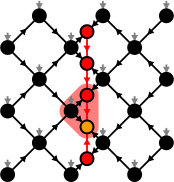
\includegraphics[scale=1]{figures/tikz/disoTPS/one_site_expectation_value/one_site_expectation_value_a.pdf}}
	\subcaptionbox{\label{fig:disoTPS_onesite_expectation_value_environment}}
	{%
		\usebox{\largestimage}
	}
	\quad\quad
	\subcaptionbox{\label{fig:disoTPS_onesite_expectation_value_computation}}
	{%
		\raisebox{\dimexpr.5\ht\largestimagea-.5\height}
		{%
			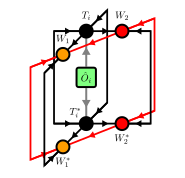
\includegraphics[scale=1.0]{figures/tikz/disoTPS/one_site_expectation_value/one_site_expectation_value_b.pdf}
		}
	}
	\caption{(a) The one-site wavefunction around a site $i$ is the sub network containing the site tensor $T_i$ and the two connected auxillary tensors. (b) The computation of a single site expectation value reduces to the shown contraction over the one-site wavefunction, its complex conjugate, and the one-site operator $\hat{O}_i$.}
	\label{fig:disoTPS_onesite_expectation_value}
\end{figure}
Similar to MPS and isoTPS, disoTPS allow for the fast computation of expectation values of local operators. The expectation value $\left\langle\Psi\right|\hat{O}_i\left|\Psi\right\rangle$ of a one-site operator $\hat{O}_i$ acting on site $i$ can be computed as follows: First, the orthogonality center is moved next to site $i$. We then define the \textit{one-site wavefunction} as the sub-network containing the site tensor $T_i$ and the two connected $W$-tensors. Note that the one-site wavefunction is connected to its environment only by bonds with incoming arrows. Next the wavefunction is contracted with its complex conjugate, sandwiching the operator $\hat{O}_i$ between the two. Due to the isometry condition, this reduces to a contraction of only the one-site wavefunction, its complex conjugate, and the operator $\hat{O}_i$, as shown in figure \ref{fig:disoTPS_onesite_expectation_value}. This contraction has a computational cost scaling as $\mathcal{O}\left(\chi^3 D^3 + D^6d^2\right) = \mathcal{O}(D^6)$ and gives as result the desired expectation value. \par
\begin{figure}
	\centering
	% Store largest image in a box
	\savebox{\largestimage}{\includegraphics[scale=1]{figures/tikz/disoTPS/two_site_expectation_value/two_site_expectation_value_a.pdf}}
	\subcaptionbox{\label{fig:disoTPS_twosite_expectation_value_environment}}
	{%
		\usebox{\largestimage}
	}
	\quad\quad
	\subcaptionbox{\label{fig:disoTPS_twosite_expectation_value_computation}}
	{%
		\raisebox{\dimexpr.5\ht\largestimage-.5\height}
		{%
			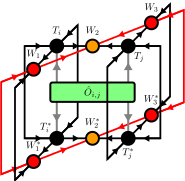
\includegraphics[scale=1.0]{figures/tikz/disoTPS/two_site_expectation_value/two_site_expectation_value_b.pdf}
		}
	}
	\caption{(a) The two-site wavefunction around neighboring sites $i$ and $j$ is the sub network containing the site tensors $T_i$ and $T_j$ and the three connected auxillary tensors. (b) The computation of a two-site expectation value reduces to the shown contraction over the two-site wavefunction, its complex conjugate, and the two-site operator $\hat{O}_{i,j}$.}
	\label{fig:disoTPS_twosite_expectation_value}
\end{figure}
The expectation value $\left\langle\Psi\right|\hat{O}_{i,j}\left|\Psi\right\rangle$ of a two-site bond operator $\hat{O}_{i,j}$ acting on two neighbouring sites $i$ and $j$ can be computed similarly. First, the orthogonality center is moved such that it sits in the middle of the bond connecting sites $i$ and $j$. The \textit{two-site wavefunction} is then defined as the subnetwork containing the two site tensors $T_i$ and $T_j$ and three $W$-tensors as shown in figure \ref{fig:disoTPS_twosite_expectation_value}, such that again all legs connecting the subnetwork to its environment are only decorated with arrows pointing towards the two-site wavefunction. The computation of the expectation value then reduces to the contraction of only the two-site wavefunction with its complex conjugate and the bond operator $\hat{O}_{i,j}$. The computational cost of this contraction scales as $\mathcal{O}\left(\chi^3D^3d^2\right) = \mathcal{O}(D^6)$.

\section{Yang-Baxter Move}
\label{sec:disoTPS_yang_baxter_move}
\begin{figure}
	\centering
	\includegraphics[width=0.9\textwidth]{figures/Tensor_Networks/disoTPS_moving_ortho_surface.jpeg}
	\caption{Two YB-moves are used to shift the orthogonality hypersurface one column to the right. In the last step, the orthogonality center can be moved across the $T$-tensor by contracting the two tensors and performing a QR-decomposition.}
	\label{fig:disoTPS_moving_ortho_surface}
\end{figure}
Most algorithms implemented on disoTPS require an efficient procedure for moving the orthogonality surface, where the error introduced by this procedure should be as small as possible. For isoTPS, the current best procedure is given by the Moses Move, followed by an optional variational optimization. \par
In analogy to the MM we look for a procedure to iteratively shift the orthogonality surface through one column of $T$-tensors as shown in figure \figref{fig:disoTPS_moving_ortho_surface}. A single iteration of this process is shown in figure \figref{fig:disoTPS_YB_move_closeup}. The two tensors $W_1$ and $W_2$, which are part of the orthogonality hypersurface, are "pulled through" the site tensor $T$, resulting in the updated tensors $T^\prime$, $W_1^\prime$ and $W_2^\prime$. To keep the isometric structure of the network, $T^\prime$ and $W_1^\prime$ must be isometries, while $W_2^\prime$ must be a tensor of norm one (the new orthogonality center). Due to the visual similarity to the Yang-Baxter equation we call this procedure the \textit{Yang-Baxter} (YB) move. \par
We denote the state represented by the disoTPS before the YB move by $\left|\Psi\right\rangle = \left|\Psi\left(W_1, W_2, T\right)\right\rangle$ and the state after the YB move by $\left|\Psi^\prime\right\rangle = \left|\Psi^\prime\left(W_1^\prime, W_2^\prime, T^\prime\right)\right\rangle$. One can think of the YB move as an optimization problem
\begin{equation}
	\label{eq:disoTPS_YB_move_standard}
	\left(T^\prime_\text{opt},W_{1,\text{opt}}^\prime,W_{2,\text{opt}}^\prime\right) = \underset{T^\prime,W_1^\prime,W_2^\prime}{\argmin}\left\lVert \left|\Psi\right\rangle - \left|\Psi^\prime\right\rangle\right\rVert_\text{F}
\end{equation}
under the constraints
\begin{equation}
	\label{eq:disoTPS_YB_move_constraints}
	T^{\prime\dagger}T^\prime = \id, \quad W_1^{\prime\dagger}W_1^\prime = \id, \quad \left\lVert W_2^\prime \right\rVert_\text{F} = 1.
\end{equation}
We further rewrite the error of the YB move as
\begin{equation}
	\label{eq:disoTPS_YB_move_rewritten_error}
	\begin{split}
		\left\lVert \left|\Psi\right\rangle - \left|\Psi^\prime\right\rangle \right\rVert_\text{F} =& \sqrt{\left\langle\Psi\middle|\Psi\right\rangle + \left\langle\Psi^\prime\middle|\Psi^\prime\right\rangle - 2\Re\left\langle\Psi\middle|\Psi^\prime\right\rangle} \\
		=& \sqrt{2 - 2\Re\left\langle\Psi\middle|\Psi^\prime\right\rangle},
	\end{split}
\end{equation}
where in the second step we used the fact that the wave function is normalized to one, $\left\langle\Psi\middle|\Psi\right\rangle = \left\langle\Psi^\prime\middle|\Psi^\prime\right\rangle = 1$. It follows that the optimization problem of minimizing the error becomes the problem of maximizing the overlap
\begin{equation}
	\label{eq:disoTPS_YB_move_alternative_formulation}
	\left(T^\prime_\text{opt},W_{1,\text{opt}}^\prime,W_{2,\text{opt}}^\prime\right) = \underset{T^\prime,W_1^\prime,W_2^\prime}{\text{argmax}}\Re\left\langle\Psi\middle|\Psi^\prime\right\rangle
\end{equation}
under the constraints \eqref{eq:disoTPS_YB_move_constraints}. Because the only tensors that are changed by the YB move are $W_1$, $W_2$ and $T$ and the three tensors make up a subregion of the full network with only incoming arrows, we can use the isometry condition and the computation of the overlap reduces to a contraction of only six tensors as shown in figure \figref{fig:YB_move_iterate_polar_overlap}.\par
\begin{figure}
	\centering
	\includegraphics[width=0.9\textwidth]{figures/Tensor_Networks/YB_move_closeup.jpeg}
	\caption{The Yang-Baxter (YB) move is the procedure of "pulling" two auxillary tensors $W_1$ and $W_2$ through a site tensor $T$.}
	\label{fig:disoTPS_YB_move_closeup}
\end{figure}
In the following, we present two explicit algorithms for performing the YB move. The first algorithm (see section \ref{sec:YB_move_iterative_local_optimization}) is an iterative optimization using local updates respecting the constraints. The second algorithm (see section \ref{sec:YB_move_svd_disentangle}) is a tripartite decomposition with disentangling similar to the tripartite decomposition used in the MM. In section \ref{sec:YB_move_comparison} we will compare the two algorithms.

\subsection{Iterative optimization with local updates}
\label{sec:YB_move_iterative_local_optimization}
To solve the constrained optimization problem \eqref{eq:disoTPS_YB_move_alternative_formulation} we proceed by maximizing the overlap while only varying the parameters of one of the three tensors $T^\prime$, $W_1^\prime$ or $W_2^\prime$, treating all other tensors as constant. For example, let us keep $W_1^\prime$ and $W_2^\prime$ fixed and optimize $T^\prime$. We first contract all tensors except $T^\prime$ into an environment $E$ as shown in figure \figref{fig:YB_move_iterate_polar}(b). We can then write the optimization problem as
\begin{equation}
	T^\prime_\text = \underset{T^{\prime\dagger}T = \id}{\argmax} \Re\left\langle\Psi\middle|\Psi^\prime\right\rangle = \underset{T^{\prime\dagger}T = \id}{\argmax}\Re\left\langle T^\prime, E\right\rangle_\text{F} = \underset{T^{\prime\dagger}T = \id}{\argmax}\Re\Tr\left(T^{\prime\dagger}E\right).
\end{equation}
This problem is known as the \textit{orthogonal Procrustes problem} and permits the closed form solution $T^\prime_\text{opt} = UV^\dagger$, where $U$ and $V$ are computed using the SVD $E = USV^\dagger$. For the derivation of this solution see appendix \ref{sec:orthogonal_procrustes_problem}. The tensors $W_1^\prime$ and $W_2^\prime$ can be optimized similarly. The full algorithm is then performed by sweeping over the three tensors, optimizing them iteratively until convergence. Tensor diagrams for the algorithm are shown in figure \figref{fig:YB_move_iterate_polar}. We discuss one iteration of the algorithm in more detail:
\begin{enumerate}
	\item We contract all tensors except $T^\prime$ into an environment $E$ and perform an SVD $E = USV$. The tensor $T^\prime$ is then updated as $T^\prime\leftarrow UV^\dagger$. See figure \figref{fig:YB_move_iterate_polar}(b).
	\item We contract all tensors except $W_1^\prime$ into an environment $E$ and perform an SVD $E = USV$. The tensor $W_1^\prime$ is then updated as $W_1^\prime\leftarrow UV^\dagger$. See figure \figref{fig:YB_move_iterate_polar}(c).
	\item We contract all tensors except $W_2^\prime$ into an environment $E$. The tensor $W_1^\prime$ is then updated as $W_1^\prime\leftarrow E/\left\lVert E\right\rVert$. See figure \figref{fig:YB_move_iterate_polar}(d).
\end{enumerate}
These three steps are repeated until a termination criterion is met, for example until the decrease in error after one iteration is smaller than a given threshold or if a given maximum number of iterations is exceeded.
\todo{Discuss complexity and initialization details!}
\begin{figure}
	\centering
	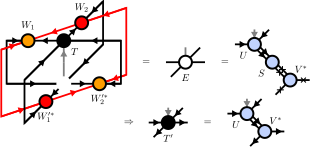
\includegraphics[scale=1]{figures/tikz/disoTPS/yang_baxter_move_iterative/yang_baxter_move_iterative_a.pdf}
	\caption{The cost function of the optimization problem \eqref{eq:disoTPS_YB_move_alternative_formulation} can be computed as a contraction of only six tensors.}
	\label{fig:YB_move_iterate_polar_overlap}
\end{figure}
\begin{figure}
	\centering
	\begin{subfigure}[c]{0.85\textwidth}
		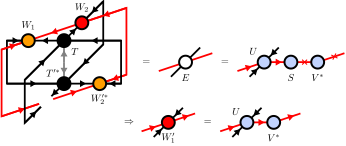
\includegraphics[scale=1]{figures/tikz/disoTPS/yang_baxter_move_iterative/yang_baxter_move_iterative_b.pdf}
		\caption{}\label{fig:YB_move_iterate_polar_optimize_T}
	\end{subfigure}
	\begin{subfigure}[c]{0.85\textwidth}
		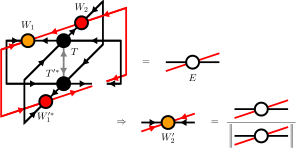
\includegraphics[scale=1]{figures/tikz/disoTPS/yang_baxter_move_iterative/yang_baxter_move_iterative_c.pdf}
		\caption{}\label{fig:YB_move_iterate_polar_optimize_W1}
	\end{subfigure}
	\begin{subfigure}[c]{0.85\textwidth}
		\includegraphics[scale=1]{figures/tikz/disoTPS/yang_baxter_move_iterative/yang_baxter_move_iterative_d.pdf}
		\caption{}\label{fig:YB_move_iterate_polar_optimize_W2}
	\end{subfigure}%
	\caption{(a) The tensor $T^\prime$ can be updated similarly by contracting all tensors except $T^\prime$ into the environment $E$ and isometrizing $E$ using an SVD. (b) The tensor $W_1^\prime$ can be updated by contracting all tensors except $W_1^\prime$ into the environment $E$, which is subsequently isometrized using an SVD. (c) To optimize the tensor $W_2^\prime$, all tensors except $W_2^\prime$ are contracted into the environment $E$. The updated tensor is then given as $W_2^\prime = E/\lVert E\rVert$.}
	\label{fig:YB_move_iterate_polar}
\end{figure}


\subsection{Tripartite decompositon using an SVD and disentangling}
\label{sec:YB_move_svd_disentangle}
Alternatively, the constrained optimization problem \eqref{eq:YB_isoTPS_YB_move_standard} can be solved via two successive SVDs with an optional disentangling prodcedure with the goal of reducing the truncation error or some entanglement measure. This is is a similar algorithm to the one used for the MM in isoTPS \cite{cite:isometric_tensor_network_states_in_two_dimensions, cite:efficient_simulation_of_dynamics_in_two_dimensional_quantum_spin_systems}, compare Section \ref{sec:tensors_and_tensor_networks_isometric_tensor_product_states_in_2D}. The algorithm is sketched in Figure \figref{fig:yb_move_svd_disent} and is made up of three main steps.
\begin{enumerate}
	\item We start by contracting the tensors $T$, $W_1$ and $W_2$ into a single tensor $\Psi$ at a cost of $\mathcal{O}(\chi^3D^4+\chi^2D^6d) = \mathcal{O}(D^8d)$. This tensor is then split from left to right via a truncated SVD
	\begin{equation}
		\Psi = ASV^\dagger = A(SV^\dagger) \eqqcolon A\theta
	\end{equation}
	as shown in Figure \figref{fig:yb_move_svd_disent_a}. Here, the bond connecting $A$ and $\theta$ has a bond dimension of $\min(dD^2, \chi^2D^2)$. The bond dimension is truncated to $D^2$. The cost of the SVD is $\mathcal{O}(\chi^2D^6d^2) = \mathcal{O}(D^8d^2)$.
	\item Next, we split the index of the bond connecting $A$ and $\theta$ into two indices of dimension $D$ each, see Figure \figref{fig:yb_move_svd_disent_b}. To proceed, we note that there exists a degree of freedom on the bonds connecting $A$ and $\theta$: A unitary $U$ and its adjoint can be inserted as shown in the second step of Figure \figref{fig:yb_move_svd_disent_b} without changing the result of the contraction
	\begin{equation}
		AU^\dagger U\theta = (AU^\dagger)(U\theta) \eqqcolon T^\prime \tilde{\theta}.
	\end{equation}
	The unitary $U$ can be chosen to minimize the truncation error of the next step by \textit{disentangling} the tensor $\theta$. We will discuss procedures of finding such a \textit{disentangling unitary} $U$ on the next page.
	\item In the last step, the tensor $\tilde{\theta}$ is split vertically into $W_1^\prime$ and $W_2^\prime$ using a truncated SVD as shown in Figure \figref{fig:yb_move_svd_disent_c}. The computational cost of this SVD scales as $\mathcal{O}(\chi^3D^6) = \mathcal{O}(D^9)$. Here, the bond dimension is truncated to $\chi$. We end up with the three tensors $T^\prime$, $W_1^\prime$ and $W_2^\prime$, completing the YB move.
\end{enumerate}
\begin{figure}
	\centering
	\subcaptionbox{\label{fig:yb_move_svd_disent_a}}
	{%
		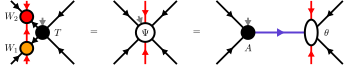
\includegraphics[scale=1.0]{figures/tikz/YB_isoTPS/yang_baxter_move_svd/yang_baxter_move_svd_a.pdf}
	}
	\par\bigskip
	\subcaptionbox{\label{fig:yb_move_svd_disent_b}}
	{%
		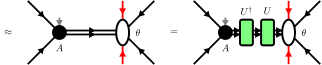
\includegraphics[scale=1.0]{figures/tikz/YB_isoTPS/yang_baxter_move_svd/yang_baxter_move_svd_b.pdf}
	}
	\par\bigskip
	\subcaptionbox{\label{fig:yb_move_svd_disent_c}}
	{%
		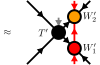
\includegraphics[scale=1.0]{figures/tikz/YB_isoTPS/yang_baxter_move_svd/yang_baxter_move_svd_c.pdf}
	}
	\caption{The YB move consists of three steps (a), (b) and (c) as explained in the text.}
	\label{fig:yb_move_svd_disent}
\end{figure}
Before we discuss the disentangling procedure, two comments about step 2 of the above algorithm are in order. First, there exists a degree of freedom for splitting the bond index, because applying the same permutations to the columns of $A$ and rows of $\theta$ does not change the result of contracting the network. However, this degree of freedom is fixed by the disentangling process, making the exact permutation of the bond splitting irrelevant. Second, note that near the edges of the lattice it can happen that the matrixized tensor $\Psi$ has $\tilde{\chi} < D^2$ rows. In this case, the bond dimension after the SVD will also be $\tilde{\chi}$ and we cannot simply split the bond into two bonds of dimension $\chi_1=\chi_2=D$. Instead, we choose a splitting $\chi_1 \le D$, $\chi_2 \le D$ such that $\chi_1\cdot\chi_2$ is maximized, while it must still hold $\chi_1\cdot\chi_2\le\tilde{\chi}$. We additionally prefer equal splittings $\chi_1\approx\chi_2\approx\sqrt{\tilde{\chi}}$ if possible. One can find such a splitting easily by computing all possible combinations of $\chi_1$ and $\chi_2$ and keeping only the best one, which has a computational cost of $\mathcal{O}\left(\sqrt{\tilde{\chi}}\right) = \mathcal{O}\left(D\right)$. See also our implementation at \cite{cite:github_YB_isoTPS}.\par
\subsubsection*{\hspace{132pt}The Disentangling Process}
\begin{figure}
	\centering
	\includegraphics[scale=1]{figures/tikz/YB_isoTPS/theta_tilde_contraction/theta_tilde_contraction.pdf}
	\caption{The disentangling unitary $U$ is contracted with the wave function tensor $\theta$ to form $\tilde{\theta}$, which is subsequently split via an SVD $\tilde{\theta} = XSY^\dagger$. The purple legs have bond dimension $\chi D$.}
	\label{fig:disentangling_theta_definition}
\end{figure}
We will now discuss the problem of finding a good disentangling unitary $U$ for step 2 of the above algorithm, which is crucial for the performance of the YB move. The problem can be formulated as follows: Given the tensor $\theta$ that is obtained after splitting the index in step 2, find a unitary $U$ minimizing a cost function $f(U, \theta)$. In the following, let $\tilde{\theta}_{(l,i),(j,r)}$ be the $\chi D^2\times \chi D^2$ matrix that is obtained by reshaping the contraction $\tilde{\theta}_{l,i,j,r} = \sum_{i^\prime,j^\prime} U_{i,j,i^\prime,j^\prime}\theta_{l,i^\prime,j^\prime,r}$ into a matrix as shown in Figure \figref{fig:disentangling_theta_definition}. Let further $\tilde{\theta} = XSY^\dagger$ denote the SVD of $\tilde{\theta}$. We discuss two cost functions, as also done in \cite{cite:efficient_simulation_of_dynamics_in_two_dimensional_quantum_spin_systems}. The first cost function is simply given by the truncation error
\begin{equation}
	\label{eq:YB_move_disent_cost_function_truncation_error}
	f_\text{trunc}\left(U,\theta\right) = \sqrt{\sum_{\mu = \chi+1}^{\chi D^2}S_\mu^2}
\end{equation}
arising in step 3 of the YB move. Alternatively, one can think of $|\tilde{\theta}\rangle \coloneqq \sum_{(l,i), (j,r)}\tilde{\theta}_{(l,i),(j,r)}\ket{(l,i), (j, r)}$ as a bipartite state in an orthogonal basis and consider as a cost function the Rényi-entropy
\begin{equation}
	\label{eq:renyi_entropy}
	f_\text{Rényi}\left(U,\theta,\alpha\right) = \frac{1}{1-\alpha}\log\Tr\left(\rho^\alpha\right) = \frac{1}{1-\alpha}\log\left(\sum_{\mu=1}^{\chi D^2}S_\mu^{2\alpha}\right),
\end{equation}
where $\alpha\in[0,\infty)$ and $\rho = \Tr_{(j, r)}(\ket{\tilde{\theta}}\bra{\tilde{\theta}})$ is the reduced density matrix obtained by tracing out one of the subsystems, see Figure \figref{fig:disentangling_rho_definition}. 
In the last step of \eqref{eq:renyi_entropy}, we used the fact that the eigenvalues of $\rho$ are the squares of the singular values of $\tilde{\theta}$. The Rényi-entropy can be used as a measure of entanglement. It approaches the Von-Neumann entanglement entropy for $\alpha\rightarrow 1$. It can be shown that the truncation error is bounded by the Rényi-entropy if $\alpha < 1$ \cite{cite:mps_represent_ground_states_faithfully}, which is a motivation for using $f_\text{Rényi}$ as a cost function. For $\alpha > 1$ such a bond cannot generally be given. However, optimizations of Rényi-entropies with $\alpha > 1$ are often simpler to perform and still achieve good results in practice \cite{cite:isometric_tensor_network_states_in_two_dimensions, cite:efficient_simulation_of_dynamics_in_two_dimensional_quantum_spin_systems, cite:finding_purifications_with_minimal_entanglement}. Setting $\alpha = 2$ yields the Rényi-entropy
\begin{equation}
	\label{eq:renyi_entropy_alpha_2}
	f_\text{Rényi}\left(U,\theta,\alpha=2\right) = -\log\Tr\rho^2,
\end{equation}
which can easily computed by contracting the tensor network shown in Figure \figref{fig:disentangling_evenbly_vidal_algorithm_trace_rho_squared} without needing to perform an SVD \cite{cite:finding_purifications_with_minimal_entanglement}. 
\begin{figure}
	\centering
	\includegraphics[scale=1]{figures/tikz/YB_isoTPS/rho_definition/rho_definition.pdf}
	\caption{Definition of the reduced density matrix $\rho$. The purple legs have bond dimension $\chi D$.}
	\label{fig:disentangling_rho_definition}
\end{figure}
\begin{figure}
	\centering
	\subcaptionbox{\label{fig:disentangling_evenbly_vidal_algorithm_trace_rho_squared}}
	{%
		\includegraphics[scale=1]{figures/tikz/YB_isoTPS/evenbly_vidal_renyi_2/evenbly_vidal_renyi_2_a.pdf}
	}
	\quad\quad\quad\quad
	\subcaptionbox{\label{fig:disentangling_evenbly_vidal_algorithm_environment_definition}}
	{%
		\includegraphics[scale=1]{figures/tikz/YB_isoTPS/evenbly_vidal_renyi_2/evenbly_vidal_renyi_2_b.pdf}
	}
	\caption{(a) Tensor network for the computation of the cost function \eqref{eq:renyi_entropy_alpha_2}. (b) Taking out one unitary $U$, the tensor network is contracted into the environment $E$.}
	\label{fig:disentangling_evenbly_vidal_algorithm}
\end{figure}
The cost function $f_\text{Rényi}\left(U,\theta,\alpha=2\right)$ can be minimized using the Evenbly-Vidal algorithm as proposed in \cite{cite:finding_purifications_with_minimal_entanglement}. First, we rewrite the minimization problem as a maximization problem
\begin{equation}
	U_\text{opt} = \underset{U^\dagger U = \id}{\argmin} f_\text{Rényi}\left(U,\theta,\alpha=2\right) = \underset{U^\dagger U = \id}{\argmax}\Tr\rho^2.
\end{equation}
We proceed by taking one tensor $U$ out of the network $\Tr\rho^2$ and contracting all other tensors into the environment $E$ as shown in Figure \figref{fig:disentangling_evenbly_vidal_algorithm_environment_definition}. We now treat $E$ as if it were independent of $U$ and update $U\leftarrow AB^\dagger$, where $A$ and $B$ are obtained by taking the SVD $E=A\Lambda B^\dagger$. This is repeated until convergence. For details on the Evenbly-Vidal algorithm see Appendix \ref{sec:evenbly_vidal_algorithm}. In practice it is observed that this algorithm for minimizing $f_\text{Rényi}\left(U,\theta,\alpha=2\right)$ converges very quickly \cite{cite:efficient_simulation_of_dynamics_in_two_dimensional_quantum_spin_systems}. The computational cost of this algorithm is dominated by the contraction of the effective environment $E$, which scales as $\mathcal{O}(\chi^3D^6) = \mathcal{O}(D^9)$. The full cost of the algorithm is thus $\mathcal{O}(N_\text{iter}D^9)$, with $N_\text{iter}$ the number of disentangling iterations.\par
\begin{figure}
	\centering
	\includegraphics[scale=1]{figures/tikz/YB_isoTPS/riemannian_optimization/riemannian_optimization.pdf}
	\caption{In this figure, a visualization of optimization on Riemannian manifolds is given. The iterate $U_k$ (left) is updated along the search direction $\xi_k$, which is an element of the tangent space $T_{U_k}\Stiefel$. The next iterate $U_{k+1}$ is computed with the retraction $R_\xi\left(\alpha\right)$, where $\alpha\in\mathbb{R}$ is the step size. For the computation of the next search direction $\xi_{k+1}$ some algorithms need the previous search direction $\xi_k$, which must first be brought to the tangent space $T_{U_{k+1}}\Stiefel$ of the new iterate $U_{k+1}$ via the vector transport $T_{k\rightarrow k+1}\left(\xi_k\right)$.}
	\label{fig:disentangling_riemannian_optimization}
\end{figure}
Minimizing the truncation error $f_\text{trunc}\left(U,\theta\right)$ and general Rényi-entropies $f_\text{Rényi}\left(U,\theta,\alpha\neq2\right)$ is a harder problem. We follow the approach of \cite{cite:isometric_tensor_network_states_in_two_dimensions, cite:efficient_simulation_of_dynamics_in_two_dimensional_quantum_spin_systems} and use Riemannian optimization \cite{cite:optimization_on_matrix_manifolds, cite:optimization_techniques_on_riemannian_manifolds, cite:riemannian_optimization_isometric_tensor_networks, cite:riemannian_geometry_automatic_differentiation_quantum_physics, cite:pymanopt} to solve the optimization problem. The idea of Riemannian optimization is to generalize common optimization algorithms that are defined in Euclidian vector spaces, such as Gradient Descent or Conjugate Gradients, to Riemannian manifolds. The set of all isometric matrices of shape $n\times m$ is a Riemannian manifold called the Stiefel manifold $\Stiefel$. A special case is the set of all unitary matrices of shape $n\times n$, $U(n)=\text{St}(n, n)$, over which we want to optimize here. Riemannian optimization over the Stiefel manifold is discussed in more detail in Appendix \ref{app:riemannian_optimization_of_isometries}. \par
A typical optimization algorithm iteratively improves an iterate $U_k\in\Stiefel$, $k=1,2,\dots$ until a local minimum of the cost function $f$ is found. In Riemannian optimization, the gradient of the cost function $\nabla f\left(U_k\right)$ is restricted to the tangent space $T_{U_k}\Stiefel$ of the iterate $U_k$ \cite{cite:optimization_on_matrix_manifolds}, which we visualize in Figure \figref{fig:disentangling_riemannian_optimization}. The gradient can be computed either analytically or via automatic differentiation \cite{cite:riemannian_geometry_automatic_differentiation_quantum_physics, cite:pymanopt}. Optimization algorithms typically compute a search direction $\xi_k\in T_{U_k}\Stiefel$ and a step size $\alpha_k \in \mathbb{R}$ from the gradient. In an optimization algorithm defined on an Euclidean vector space one would then move along this direction as
\begin{equation}
	\tilde{U}_{k+1} = U_k + \alpha_k\xi_k.
\end{equation}
However, $\tilde{U}_{k+1}$ is in general not an element of the manifold. To ensure $U_{k+1}\in\Stiefel$, one can introduce a \textit{retraction} $R_{\xi_k}:\mathbb{R}\to\Stiefel$ \cite{cite:optimization_on_matrix_manifolds}. One can think of $R_{\xi_k}(\alpha_k)$ as moving along the direction of $\xi_k$ while staying on the manifold. As $\alpha_k$ increases, we move further along the path defined by the retraction, with $R_{\xi_k}(0) = U_k$, see Figure \figref{fig:disentangling_riemannian_optimization}. Different retractions can be chosen, varying by how well they perform in optimization problems and by how hard they are to compute. Here we choose the retraction
\begin{equation}
	R_{\xi_k}(\alpha_k) = \qf\left(U_k + \alpha_k\xi_k\right),
\end{equation}
where $\qf\left(A\right)$ is the Q-factor of the QR-decomposition $A = QR$. This retraction is particularly easy to compute and yields good results in practice. \par
Many optimization algorithms such as Conjugate Gradients require gradients or search directions from previous iterates for computing a search direction at the current iterate. In Riemannian optimization, one must first bring these gradients and search directions from the tangent spaces of previous iterates to the tangent space of the current iterate. This is handled by a so-called \textit{vector transport} $T_{k\rightarrow k+1}\left(\xi_k\right)$ \cite{cite:optimization_on_matrix_manifolds}, see Figure \figref{fig:disentangling_riemannian_optimization}. \par
Finally, for optimization algorithms of second order such as the trust-region method, one needs to generalize the notion of the Hessian-vector product to Riemannian manifolds. This generalization is given by the \textit{Riemannian connection} \cite{cite:optimization_on_matrix_manifolds}. For the Stiefel manifold the Hessian-vector product is simply given by projecting the Hessian-vector product of the embedding euclidean vector space $\mathbb{C}^{n\times p}$ to the tangent space. \par
We use two algorithms for solving the disentangling optimization problem, Conjugate Gradients (CG) and the Trust-Region Method (TRM). CG uses the accumulated gradients of previous iterations to compute an improved search direction, trying to achieve superlinear convergence. CG is discussed in more details in Appendix \ref{sec:conjugate_gradients}. The TRM approximates the cost function around the current iterate through a quadratic function using the Hessian-vector product. This approximate cost function is then minimized within a region of radius $\Delta\in\mathbb{R}$ using truncated Conjugate Gradients (tCG), which converges quickly for the quadratic approximation. Depending on the quality of the approximation at the current iterate one can then shrink or enlarge the trust region. TRM is able to achieve local superlinear convergence while still retaining desired global convergence properties \cite{cite:optimization_on_matrix_manifolds} and can be thought of as an improved version of Newton's method. For more details, see Appendix \ref{sec:trust_region_method}. \par
The gradients and Hessian-vector products of the cost functions \eqref{eq:YB_move_disent_cost_function_truncation_error} and \eqref{eq:renyi_entropy} can be computed analytically with a computational cost of $\mathcal{O}(D^9)$, see Appendix \ref{app:computation_of_gradient_and_hvp_for_riemannian_optimization} for a derivation.
\subsubsection*{\hspace{70pt}Approximate Gradients and Hessian-Vector Products}
\begin{figure}
	\centering
	\subcaptionbox{\label{fig:approximate_svd_overlap}}
	{%
		
\includegraphics[scale=1]{figures/tikz/YB_isoTPS/approximate_svd/approximate_svd_a.pdf}
	}
	\par\bigskip
	\subcaptionbox{\label{fig:approximate_svd_first_step}}
	{%
		
\includegraphics[scale=1]{figures/tikz/YB_isoTPS/approximate_svd/approximate_svd_b.pdf}
	}
	\par\bigskip
	\subcaptionbox{\label{fig:approximate_svd_second_step}}
	{%
		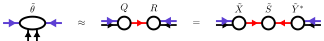
\includegraphics[scale=1]{figures/tikz/YB_isoTPS/approximate_svd/approximate_svd_c.pdf}
	}
	\par\bigskip
	\subcaptionbox{\label{fig:approximate_svd_final_step}}
	{%
		\includegraphics[scale=1]{figures/tikz/YB_isoTPS/approximate_svd/approximate_svd_d.pdf}
	}
	\caption{In this figure we draw tensor diagrams for the approximate SVD. First, an approximate QR-decomposition is performed by minimizing the inner product $\langle\tilde{\theta},QR\rangle_\text{F}$ (a). This can be done by iteratively updating the $R$-tensor (b) and the $Q$-tensor (c). We finish the approximate SVD by performing a standard SVD on the tensor $\Lambda$, which has reduced bond dimension (d).}
	\label{fig:approximate_qr_decomposition}
\end{figure}
The cost of both CG and the TRM are dominated by the computation of the gradient and Hessian-vector product, particularly by the SVD $\tilde{\theta} = XSY^\dagger$ and contractions involving the tensors $X$ and $Y$. The reason for this is the large bond dimension $\chi D^2$ of the bond connecting $X$ and $Y$, see Figure \figref{fig:disentangling_theta_definition}. We thus propose to approximate the gradient and Hessian-vector product by instead performing an approximate SVD $\tilde{\theta} \approx \tilde{X}\tilde{S}\tilde{Y}^\dagger$, where we only keep $\chi$ of the $\chi D^2$ singular values. The algorithm for performing this approximate SVD is inspired by \cite{cite:fast_time_evolution_of_mps_using_qr}, where a similar algorithm was used to speed up TEBD updates for MPS. We sketch the algorithm in Figure \figref{fig:approximate_qr_decomposition}. First, an approximate QR-decomposition $\tilde{\theta} = QR$ with $Q\in\mathbb{C}^{\chi D^2\times\chi}$ and $R\in\mathbb{C}^{\chi\times\chi D^2}$ is performed by variationally minimizing the distance $\lVert \tilde{\theta} - QR \rVert$, which is equivalent to maximizing the real part of the overlap $\Re\langle\tilde{\theta},QR\rangle_\text{F}$. The overlap is shown as a tensor diagram in Figure \figref{fig:approximate_svd_overlap}. It can be maximized by alternatingly optimizing the tensors $Q$ and $R$ as shown in Figures \figref{fig:approximate_svd_first_step} and \figref{fig:approximate_svd_second_step} respectively, which costs $\mathcal{O}(\chi^3D^4) = \mathcal{O}(D^7)$ per iteration. A standard SVD is then performed on the $R$-factor of the approximate QR-decomposition as $R = A\tilde{S}\tilde{Y}^\dagger$, and the contraction $\tilde{X} = QA$ finalizes the decomposition, see Figure \figref{fig:approximate_svd_final_step}. In total, the cost of the approximate SVD is $\mathcal{O}(N_\text{svd}D^7)$, with $N_\text{svd}$ the number of iterations, instead of $\mathcal{O}(D^9)$ for a full SVD. It is observed that the variational minimization that is used to compute the approximate SVD converges very quickly in practice, especially if a good initialization is chosen. As the iterates $U_k$ are expected to only change slightly in each iteration of CG or TRM, one can simply use the result $Q, R$ obtained in the approximate QR-decomposition of the previous iteration as initialization for the next iteration. We observe that the variational optimization in practice converges in less than $5$ iterations. \par
Using the approximate SVD, we were able to decrease the cost of the gradient computation from $\mathcal{O}(D^9)$ to $\mathcal{O}(D^8 + N_\text{svd}D^7)$. Moreover, through caching of the most costly contraction, the cost of the tCG sub-procedure that is called in every iteration of the TRM can be brought down from $\mathcal{O}(N_\text{tCG}D^9)$ to $\mathcal{O}(D^8+N_\text{svd}D^7 + N_\text{tCG} D^7)$, where $N_\text{tCG}$ is the maximum number of iterations for which the tCG sub-procedure is run. Finally, one can also use an approximate SVD for the final vertical splitting performed in step 3 of the YB move after the disentangling is complete, improving the scaling from $\mathcal{O}(D^9)$ to $\mathcal{O}(N_\text{svd}D^7)$. To summarize, we list the computational complexity of all discussed algorithms for the YB move in Table \figref{table:computational_complexity_YB_move}.
\begin{table}
	\begin{tabular}{ l | l }
		Evenbly-Vidal style iterative optimization & $\mathcal{O}(N_\text{iter}D^8)$ \\ \\[-1em]
		\hline \\[-1em]
		SVD splitting & $\mathcal{O}(D^9)$ \\ \\[-1em]
		\hline \\[-1em]
		approximate SVD splitting & $\mathcal{O}(D^8 + N_\text{svd}D^7)$ \\ \\[-1em]
		\hline
		\hline \\[-1em]
		Evenbly-Vidal Rényi-2 disentangler  & $\mathcal{O}(N_\text{iter}D^9)$ \\ \\[-1em]
		\hline \\[-1em]
		CG disentangler & $\mathcal{O}(N_\text{iter}D^9)$ \\ \\[-1em]
		\hline \\[-1em]
		TRM disentangler & $\mathcal{O}(N_\text{iter}N_\text{tCG}D^9)$ \\ \\[-1em]
		\hline \\[-1em]
		approximate CG disentangler & $\mathcal{O}(N_\text{iter}(D^8 + N_\text{svd}D^7))$ \\ \\[-1em]
		\hline \\[-1em]
		approximate TRM disentangler & $\mathcal{O}(N_\text{iter}(D^8 + N_\text{svd}D^7 + N_\text{tCG}D^7))$ \\
	\end{tabular}
	\caption{In this table we summarize the complexity scaling of the different discussed algorithms for performing the YB move. The scaling of the Rényi-entropy and truncation error disentangling is the same, but with different prefactors.}
	\label{table:computational_complexity_YB_move}
\end{table}
\subsubsection*{\hspace{105pt}Comparison of Different Disentanglers}
We will now compare the different algorithms for solving the disentangling problem.
\input{figures/plots/YB_isoTPS/yb_move_disentangling_renyi_2.tex}
\input{figures/plots/YB_isoTPS/yb_move_disentangling_renyi_0.5_trunc_error.tex}
For this comparison we select the YB move environment $\left\{W_1, W_2, T\right\}$ that was already used to discuss the convergence behaviour of the iterative algorithm in Section \ref{sec:YB_move_iterative_local_optimization}. The results on other YB environments agree qualitatively with the results we present here. The bond dimensions chosen for the YB-isoTPS are $D = 4$, $\chi = 24$. \par
We first test the Evenbly-Vidal algorithm optimizing the Rényi-entropy with $\alpha = 2$, see Figure \figref{fig:YB_isoTPS_disentangling_evenbly_vidal_renyi_2}. The algorithm converges very quickly after only $\approx 20$ iterations. The convergence speed depends drastically on the initialization of the disentangling unitary. We find that a initialization based on an SVD of $\theta$ works best, see our implementation \cite{cite:github_YB_isoTPS}. This initialization procedure was introduced for the MM for isoTPS \cite{cite:isometric_tensor_network_states_in_two_dimensions, cite:efficient_simulation_of_dynamics_in_two_dimensional_quantum_spin_systems}. \par
Next, we look at the performance of CG and TRM optimizing the Rényi-entropy with $\alpha = 1/2$ and the truncation error in Figures \figref{fig:YB_isoTPS_disentangling_cg_trm_renyi_0.5} and \figref{fig:YB_isoTPS_disentangling_cg_trm_truncation_error} respectively. In both cases we observe that the TRM leads to a faster decrease in the cost function for the same number of iterations compared to CG. Remarkably, the approximate versions of both CG and TRM perform almost as good as their exact counterparts. Again, the speed of convergence depends strongly on the initialization. Because of the quick convergence of the Evenbly-Vidal algorithm optimizing the $\alpha = 2$ Rényi-entropy, we choose its result as an initialization for the optimization algorithms using Riemannian optimization. This achieved the best results in our testing. \par
Last, we plot the cost function against the walltime of the Riemannian disentangling algorithms in Figures \figref{fig:YB_isoTPS_disentangling_cg_trm_renyi_0.5_walltime} and \figref{fig:YB_isoTPS_disentangling_cg_trm_truncation_error_walltime}. For this benchmark, the algorithms were run on an i5-12500 CPU with 6 cores. As one can see, the approximate versions of both CG and TRM run up to an order of magnitude faster while still providing a comparable minimization of the cost function. Thus, in practice, it is often better to choose a larger maximum bond dimension with the approximate disentangling algorithms instead of a smaller maximum bond dimension with the exact algorithms.


\subsection{Comparison of the two algorithms}
\label{sec:YB_move_comparison}

\section{Time Evolving Block Decimation (TEBD)}
\label{sec:disoTPS_TEBD}
We will now discuss the Time Evolving Block Decimation (TEBD) algorithm for disoTPS, which can be used for both real and imaginary time evolution. The algorithm is a generalization of TEBD for MPS, which we discussed in section \ref{sec:tensors_and_tensor_networks_matrix_product_states}. Analogeously to MPS we start with a Suzuki-Trotter decomposition, approximating the time evolution operator $U\left(\Delta t\right) = e^{-i\Delta t \hat{H}}$ by a product of bond operators $U^{[x, y]}\left(\Delta t\right)$ acting only on neighbouring sites on the bond $[x, y]$. These bond operators then must be applied to the state in the correct order, while keeping the disoTPS structure intact. We will discuss the process of applying a single bond operator $U^{[x,y]}\left(\Delta t\right)$ to the disoTPS in section \ref{sec:local_TEBD_updates}. In section \ref{sec:global_TEBD_updates} we then discuss the full TEBD algorithm.

\subsection{Local TEBD updates}
\label{sec:disoTPS_TEBD_local_updates}
\begin{figure}
	\centering
	\subcaptionbox{\label{fig:disoTPS_TEBD_five_tensor_environment}}
	{%
		\includegraphics[width=0.3\textwidth]{figures/disoTPS/disoTPS_TEBD_5_tensor_environment.jpeg}
	}
	\subcaptionbox{\label{fig:disoTPS_TEBD_contraction_definition}}
	{%
		\includegraphics[width=0.6\textwidth]{figures/disoTPS/disoTPS_TEBD_contraction_definitions.jpeg}
	}
	\caption{(a The five tensor environment of the bond on which the bond operator is to be applied. All arrows are incoming. (b) Definitions of the sub-networks $\mathcal{C}$ and $\mathcal{C}^\prime$ used in equation \eqref{eq:isoDTPS_TEBD_local_update_error}.}
	\label{fig:disoTPS_TEBD_definition_of_environment}
\end{figure}
Let us assume that the orthogonality center is positioned between the two sites on which the bond operator $\hat{U}^{[x, y]}\left(\Delta t\right)$ acts. The five tensors around the orthogonality center then make up a sub-network with only incoming arrows, see figure \figref{fig:disoTPS_TEBD_five_tensor_environment}. We call these five tensors $T_1$, $T_2$, $W_1$, $W_2$ and $W_3$. The local TEBD update can then be formulated as the following problem: Find tensors $T_1^\prime$, $T_2^\prime$, $W_1^\prime$, $W_2^\prime$ and $W_3^\prime$ satisfying the isometry constraints and minimizing the error
\begin{equation}
	\label{eq:isoDTPS_TEBD_local_update_error}
	\varepsilon_\text{trunc} = \left\lVert \hat{U}^{[x,y]}(\Delta t)|\Psi\rangle - |\Psi\rangle\right\rVert = \underset{T_1^\prime, T_2^\prime, W_1^\prime, W_2^\prime, W_3^\prime}{\argmax}\Re\langle\Psi|\hat{U}^{[x,y]}(\Delta t)|\Psi^\prime\rangle.
\end{equation}
Using the isometry condition, the overlap $\langle\Psi|\hat{U}^{[x,y]}(\Delta t)|\Psi^\prime\rangle$ can be comput by contracting the tensor network drawn in figure \figref{fig:disoTPS_TEBD_contraction_definition}. For solving this problem we again use the Evenbly-Vidal algorithm. As we already did in section \ref{sec:YB_move_iterative_local_optimization} for the YB move, we optimize one tensor at a time while keeping all other tensors fixed. This procedure is then repeated, sweeping over all five tensors until convergence is achieved. For more details on this optimization method see appendix \ref{app:riemannian_optimization_of_isometries}. Since the time step $\Delta t$ is chosen to be small, the bond operator is close to identity, $\hat{U}^{[x,y]}(\Delta t)\approx\id$. Thus, a good initialization for the tensors of the updated wavefunction $|\Psi^\prime\rangle$ are simply the tensors of the old wavefunction $|\Psi\rangle$. \par
The computational complexity of applying a local bond operator to a disoTPS with the discussed algorithm scales as $\mathcal{O}(\chi^3D^3d^2) = \mathcal{D^6}$. \todo{Talk about convergence!}

\subsection{Global TEBD updates}
\label{sec:disoTPS_TEBD_global_updates}
\begin{figure}
	\centering
	\subcaptionbox{\label{fig:disoTPS_TEBD_global_update_TEBD1_splitting}}
	{%
		\includegraphics[scale=1]{figures/tikz/disoTPS/tebd_global_update/tebd_global_update_a.pdf}
	}
	\caption{A Hamiltonian $\hat{H}$ that is a sum of nearest-neighbour operators $h^{[x,y]}$ can be split into four parts made up of operators acting only on even/odd columns and even/odd bonds along a column.}
	\label{fig:disoTPS_TEBD_global_update_TEBD1_splitting_and_TEBD2_chain}
\end{figure}
A global TEBD update evolves the state by a time $\Delta t$ and can be performed by applying local TEBD updates on all bonds. For each local TEBD update, the orthogonality center must be moved to the bond at which the update is applied. Because moving the orthogonality hypersurface can only be done approximately, the number of necessary moves should be minimized. \par
As we have already done for MPS in section \ref{sec:tensors_and_tensor_networks_matrix_product_states} let us assume that the Hamiltonian $\hat{H}$ can be written as a sum of nearest-neighbour operators. We index these nearest-neighbour operators $h^{[x, y]}$ by two integers $x$ and $y$ corresponding to the position of the orthogonality hypersurface and orthogonality center if moved to the bond on which $h^{[x,y]}$ acts. We define $x$ to increase from left to right and $y$ to increase from bottom to top, as shown in figure \figref{fig:disoTPS_TEBD_global_update_TEBD1_splitting}. The Hamiltonian can then be split into four parts by first grouping the $h^{[x,y]}$ into two sets acting only on even and odd columns respectively and then splitting each set again into terms acting only on even/odd bonds along the respective columns. We can write this as
\begin{equation}
	\label{eq:disoTPS_TEBD_splitting_local_Hamiltonian}
	\begin{split}
		\hat{H} = \sum_{x=1}^{2L_x-1} \sum_{y=1}^{2L_y-1}h^{[x,y]} &= \sum_{\substack{x\text{ even}\\y\text{ even}}} h^{[x, y]} + \sum_{\substack{x\text{ even}\\y\text{ odd}}} h^{[x, y]} + \sum_{\substack{x\text{ odd}\\y\text{ even}}} h^{[x, y]} + \sum_{\substack{x\text{ odd}\\y\text{ odd}}} h^{[x, y]} \\
		&\eqqcolon \hat{H}_1 + \hat{H}_2 + \hat{H}_3 + \hat{H}_4,
	\end{split}
\end{equation}
see also figure \figref{fig:disoTPS_TEBD_global_update_TEBD1_splitting}. The operators appearing in the sum in $\hat{H}_j$ commute with each other and thus the exponential $e^{-i\Delta t\hat{H}_j}$ factorizes into a product of bond operators $\hat{U}^{[x, y]}(\Delta t) = e^{-i\Delta t\hat{h}^{[x, y]}}$. \par
We next use a Suzuki-Trotter decomposition to approximate the time evolution operator
\begin{equation}
	\label{eq:disoTPS_TEBD_suzuki_trotter_first_order}
	\hat{U}(\Delta t) = \hat{U}^\text{TEBD1}(\Delta t) + \mathcal{O}(\Delta t^2)
\end{equation}
with
\begin{equation}
	\label{eq:disoTPS_TEBD_first_order_TEBD_operator}
	\hat{U}^\text{TEBD}(\Delta t) \coloneqq e^{-i\Delta t\hat{H}_4} e^{-i\Delta t\hat{H}_3} e^{-i\Delta t\hat{H}_2} e^{-i\Delta t\hat{H}_1}.
\end{equation}
To evolve the state $|\Psi\rangle$ in time with this first order approximation we must compute $|\Psi^\prime\rangle \approx U^\text{TEBD1}(\Delta t)|\Psi\rangle$ as a disoTPS. The procedure is sketched in figure \figref{fig:disoTPS_TEBD_global_update_applying_TEBD1}. We start in the left-most column and apply all bond operators that act on bonds along this column. The bond operators on the column are applied analogeously to the MPS algorithm: First we update all even bonds and then we update all odd bonds. Local updates are computed using the algorithm discussed in section \ref{sec:disoTPS_TEBD_local_updates}. Next, we move the orthogonality hypersurface two columns to the right and again apply all bond operators along the column. We proceed until all bond operators on even columns have been applied, in which case the orthogonality hypersurface is now positioned at its right-most position. We now sweep back to the left, applying all bond operators acting on odd columns along the way. Arriving back at the left-most column, all bonds making up $\hat{U}^\text{TEBD1}(\Delta t)$ have been applied in the correct order and the state has been evolved by time $\Delta t$. \par
\begin{figure}
	\centering
	\subcaptionbox{\label{fig:disoTPS_TEBD_global_update_applying_TEBD1}}
	{%
		\includegraphics[scale=1]{figures/tikz/disoTPS/tebd_global_update_steps/tebd_global_update_steps_a.pdf}
	}
	\par\bigskip
	\subcaptionbox{\label{fig:disoTPS_TEBD_global_update_applying_TEBD2}}
	{%
		\includegraphics[scale=1]{figures/tikz/disoTPS/tebd_global_update_steps/tebd_global_update_steps_b.pdf}
	}
	\caption{To apply a TEBD update of (b) first order and (b) second order, we sweep accross the disoTPS once from left to right and back from right to left. (a) TEBD1 applies the operators in a brick-wall fashion, while (b) TEBD2 applies the operators along a chain. \todo{The second picture should apply along a chain}}
	\label{fig:disoTPS_TEBD_global_update_applying_TEBD}
\end{figure}
We can obtain a better approximation of the time evolution operator $U(\Delta t)$ by performing a second order Suzuki-Trotter decomposition. By repeatedly applying the symmetrized decomposition
\begin{equation}
	e^{-i\varepsilon(A+B)} = e^{-i\frac{\varepsilon}{2}A}e^{-i\frac{\varepsilon}{2}A}e^{-i\varepsilon B} + \mathcal{O}(\Delta t^3)
\end{equation}
we obtain
\begin{equation}
	\begin{split}
		\label{eq:disoTPS_tebd_second_order_suzuki_trotter_decomposition}
		e^{-i\Delta t\hat{H}} &= \exp\left(-i\Delta t\sum_{x,y}\hat{h}^{[x,y]}\right) \\
		&= e^{-i\frac{\Delta t}{2}\hat{h}^{[1, 1]}} e^{-i\Delta t\left(\hat{H}-\hat{h}^{[1,1]}\right)} e^{-i\frac{\Delta t}{2}\hat{h}^{[1, 1]}} + \mathcal{O}(\Delta t^3)\\
		&= e^{-i\frac{\Delta t}{2}\hat{h}^{[1, 1]}} e^{-i\frac{\Delta t}{2}\hat{h}^{[1, 2]}} e^{-i\Delta t\left(\hat{H}-\hat{h}^{[1,1]}-\hat{h}^{[1, 2]}\right)} e^{-i\frac{\Delta t}{2}\hat{h}^{[1, 2]}} e^{-i\frac{\Delta t}{2}\hat{h}^{[1, 1]}} + \mathcal{O}(\Delta t^3)\\
		&=\cdots\\
		&= e^{-i\frac{\Delta t}{2}\hat{h}^{[1, 1]}} e^{-i\frac{\Delta t}{2}\hat{h}^{[1, 2]}} \cdots e^{-i\frac{\Delta t}{2}\hat{h}^{[1, 2]}} e^{-i\frac{\Delta t}{2}\hat{h}^{[1, 1]}} + \mathcal{O}(\Delta t^3).
	\end{split}
\end{equation}
Here, in each step we "split off" one operator $\hat{h}^{[x,y]}$ from the sum. The final result is a product of bond operators $\hat{U}^{[x,y]}(\Delta t/2))$ that must be applied from right to left. We can visualize this as a chain of bond operators that are applied along the path sketched in figure \figref{fig:disoTPS_TEBD_global_update_TEBD2_chain}. We start from the bottom left of the lattice, visiting every bond, and ending up on the top right. The same string of bond operators must then be applied backwards until arriving again at the bottom left. \par
The algorithm of applying a global update is thus similar to a TEBD update of first order. We sweep across the disoTPS once from left to right and back, applying bond operators along the way in the correct order, as visualized in figure \figref{fig:disoTPS_TEBD_global_update_applying_TEBD2}. The number of YB moves for TEBD1 and TEBD2 is the same, but the smaller Trotter error of $\mathcal{O}(\Delta t^3)$ instead of $\mathcal{O}(\Delta t^2)$ allows us to use larger time steps for TEBD2, resulting in a smaller number of YB moves per unit time. We find that the YB move is the primary source of error in practice and thus expect TEBD2 to perform much better than TEBD1. \par 
In principle, one could also go to higher decomposition orders \cite{cite:finding_exponential_product_formulas_of_higher_orders}. However, already a third order decomposition would necessitate a larger number of sweeps for applying the full update, increasing the error accumulated through YB moves. It is therefore not clear if higher order decompositions would be able to improve the method further.

	
	\chapter{Toric Code: An exactly representable Model}
	In this chapter we show that the YB-isoTPS ansatz introduced in Chapter \ref{chap:isoTPS_alternative_canonical_form} is able to exactly represent the ground state of the Toric Code Model. We first give a brief introduction to the Toric Code model in Section \ref{sec:the_toric_code_model} and show how the ground state can be derived analytically. We then discuss how this ground state can be represented as a YB-isoTPS in Section \ref{sec:representing_the_toric_code_gs_with_YB_isoTPS}.

\section{The Toric Code Model}
\label{sec:the_toric_code_model}
The Toric Code is an exactly soluble spin model with $\mathbb{Z}_2$ topological order that was introduced by Alexei Kitaev \cite{cite:fault_tolerant_quantum_computation_by_anyons}. The model is defined on the square lattice with periodic boundary conditions, where on each edge of the lattice there sits a spin-1/2 degree of freedom. Two operators are introduced, the \textit{star operators}
\begin{equation}
	\label{eq:star_operator}
	\hat{A}_+ \coloneqq \sum_{j\in+}\hat{\sigma}_j^z
\end{equation}
and the \textit{plaquette operators}
\begin{equation}
	\label{eq:plaquette_operator}
	\hat{B}_{\scalebox{0.6}{$\square$}} \coloneqq \sum_{j\in \scalebox{0.6}{$\square$}} \hat{\sigma}_j^x,
\end{equation}
where the sums are performed over the four spins connected in a star or plaquette pattern respectively (see Figure \figref{fig:toric_code_star_and_plaquette_operators}) and $\hat{\sigma}_j^x, \hat{\sigma}_j^z$ are Pauli matrices. The Hamiltonian of the Toric Code model is then defined as
\begin{equation}
	\label{eq:toric_code_hamiltonian}
	H_\text{TC} \coloneqq -\sum_+\hat{A}_+ - \sum_{\scalebox{0.6}{$\square$}}\hat{B}_{\scalebox{0.6}{$\square$}},
\end{equation}
where the sums go over all possible stars and plaquettes respectively. Because an arbitrary star and plaquette operator share either two or zero spins, all terms of the Hamiltonian commute and it is thus possible to find the ground state of the model by diagonalizing all terms simultaneously. To diagonalize the star operators $\hat{A}_+$ we choose a basis of $\hat{\sigma}_z$-eigenstates $\ket{i} \in \left\{\ket{\uparrow}, \ket{\downarrow}\right\}$ with eigenvalues $\left\langle\hat{\sigma}_z\right\rangle_i = s_i = \pm 1$ for each spin $i$. In this basis every star operator is diagonal with eigenvalues
\begin{equation}
	\label{eq:toric_code_star_operator_expectation value}
	\langle \hat{A}_+\rangle = \prod_{j\in+}s_j \in \left\{1, -1\right\}.
\end{equation}
To obtain the expectation value $\langle \hat{A}_+\rangle = 1$, the number of spins in the down state $s_j = -1$ around the vertex $+$ must be even. Basis states $\ket{s}$ that give an expectation value of $1$ for every star operator simultaneously are thus the states with an even number of down-spins around every vertex,
\begin{equation}
	\label{eq:toric_code_A_operator_condition}
	\ket{s} = \ket{s_1} \otimes \dots \otimes \ket{s_N}, \quad \prod_{j\in+}s_j = 1 \,\,\,\,\forall +.
\end{equation}
The plaquette operator $\hat{B}_{\scalebox{0.6}{$\square$}}$ acts on a basis state by flipping all spins around the plaquette $\scalebox{0.6}{$\square$}$. Because a plaquette and a star share either zero or two spins, applying an plaquette operator to a state $\ket{s}$ satisfying condition \eqref{eq:toric_code_A_operator_condition} produces a state $\ket{s^\prime}$ that again satisfies \eqref{eq:toric_code_A_operator_condition}, and applying the plaquette operator a second time produces the initial state $\ket{s}$. If we now take the equal weighted superposition $\ket{\Psi} = \left(\ket{s}+\ket{s^\prime}\right)/\sqrt{2}$, the expectation value of $\hat{B}_{\scalebox{0.6}{$\square$}}$ becomes $\langle \hat{B}_{\scalebox{0.6}{$\square$}}\rangle = 1$.
The ground state of the Hamiltonian \eqref{eq:toric_code_hamiltonian} is thus given by the equal weighted superposition of all basis states satisfying condition \eqref{eq:toric_code_A_operator_condition}. \par
One can show that the ground state can be written as
\begin{equation}
	\ket{\Psi_0} \propto \prod_{\scalebox{0.6}{$\square$}}\left(\id + \hat{B}_{\scalebox{0.6}{$\square$}}\right) \ket{\uparrow} \otimes \dots \otimes \ket{\uparrow}.
\end{equation}
Note that this is also the ground state for the model if open boundary conditions are chosen instead. \par
For periodic boundary conditions, which is equivalent to putting the model on a torus, one can further show that the ground state is fourfold topologically degenerate. To move from one degenerate section of the Hilbert space to another one must apply a string of operators, wrapping once around the torus. This is a highly non-local operation. Because perturbations are usually local, the toric code model can be interpreted as a form of hardware level error correction. The toric code is considered a topological quantum error correction code and can in theory be used for quantum memory. One can further implement quantum gates acting on the 4-dimensional ground state space by locally creating a pair of anyonic excitations, moving one of the excitations around the torus, and annihilating it with the other one \cite{cite:fault_tolerant_quantum_computation_by_anyons}. Unfortunately, the gates that can be implemented as such do not form a complete state set and thus do not allow for universal quantum computing. Nevertheless, the Toric code is an important model for the study of topological order and anyonic excitations.
\begin{figure}
	\centering
	\includegraphics[scale=1]{figures/tikz/toric_code/toric_code_general/toric_code_general.pdf}
	\caption{The Toric Code model is defined on the square lattice with spin-1/2 degrees of freedom living on the edges. the star and plaquette operators \eqref{eq:star_operator} and \eqref{eq:plaquette_operator} act on the four spins arranged in a star or plaquette shape respectively.}
	\label{fig:toric_code_star_and_plaquette_operators}
\end{figure}


\section{Representing the Toric Code Ground State with YB-isoTPS}
\label{sec:representing_the_toric_code_gs_with_YB_isoTPS}
We will now derive the YB-isoTPS corresponding to the Toric Code ground state on a square lattice with open boundary condition. We choose rough boundary conditions \cite{cite:models_for_gapped_boundaries_and_domain_walls}, fixing all boundary spins to the state $\left(\ket{\uparrow} + \ket{\downarrow}\right)/\sqrt{2}$. As shown in \cite{cite:isometric_tensor_network_representation_of_string_net_liquids}, the Toric Code ground state can be represented exactly as a PEPS with bond dimension $D = 2$. One can construct such a PEPS by first doubling the Hilbert space on each edge as $\ket{s_i} \rightarrow \ket{s_i}\otimes\ket{s_i}$, which we show in Figure \figref{fig:toric_code_doubling_dof}. In the PEPS representation the physical degrees of freedom on each edge in the bulk are then carried by two identical tensors $\delta^\text{B}\in\mathbb{R}^{2\times2\times2}$,
\begin{equation}
	\delta^\text{B}{i,\alpha,\beta} = \begin{cases}
		1 &\text{if }i=\alpha=\beta\\
		0 &\text{else}
	\end{cases},
\end{equation}
as shown in Figure \figref{fig:toric_code_PEPS_representation_tensor_definitions}. The boundary spins are represented by tensors $\delta_E\in\mathbb{R}^{2\times2}$,
\begin{equation}
	\delta^\text{E}{i,\alpha} = \begin{cases}
		1 &\text{if }i=\alpha\\
		0 &\text{else}
	\end{cases}.
\end{equation}
We proceed by associating each vertex with the spins on the four connected edges and contract the corresponding tensors $\delta^\text{B}$ and $\delta^\text{E}$ with a tensor $T\in\mathbb{R}^{2\times2\times2\times2}$ that is placed on each vertex,
\begin{equation}
	T_{i,j,k,l} = \begin{cases}
		1 & \text{if } (i+j+k+l)\,\text{mod}\,2 = 0 \\
		0 & \text{else}
	\end{cases}.
\end{equation}
This tensor ensures that all states with an odd number of down spins around a vertex have an amplitude of zero, satisfying condition \eqref{eq:toric_code_A_operator_condition}. \par
\begin{figure}
	\centering
	\savebox{\largestimage}{\includegraphics[scale=1]{figures/tikz/toric_code/peps_representation/peps_representation_a.pdf}}
	\subcaptionbox{\label{fig:toric_code_doubling_dof}}
	{%
		\usebox{\largestimage}
	}
	\quad
	\subcaptionbox{\label{fig:toric_code_PEPS_representation_tensor_definitions}}
	{%
		\raisebox{\dimexpr.5\ht\largestimage-.5\height}
		{%
			\includegraphics[scale=1]{figures/tikz/toric_code/peps_representation/peps_representation_b.pdf}
		}
	}
	\quad
	\subcaptionbox{\label{fig:toric_code_PEPS_representation}}
	{%
		\raisebox{\dimexpr.5\ht\largestimage-.5\height}
		{%
			\includegraphics[scale=1]{figures/tikz/toric_code/peps_representation/peps_representation_c.pdf}
		}
	}
	\caption{(a) To represent the Toric Code ground state as a PEPS we start by doubling the local degrees of freedom on each edge in the bulk. Bulk spins are denoted in red, while boundary spins are coloured blue. (b) Tensor diagrams of the tensors $\delta^\text{B}$, $\delta^\text{E}$ and $T$ introduced in the text. (b) The PEPS representation of the Toric Code ground state before contracting the tensors at each vertex, made up from the tensors (b).}
	\label{fig:toric_code_doubling_dof_and_PEPS_representation}
\end{figure}
We arrive at the PEPS in Figure \figref{fig:toric_code_PEPS_representation}. Each basis state satisfying condition \eqref{eq:toric_code_A_operator_condition} results in the same amplitude when contracting the PEPS, while basis states violating the condition vanish. Thus, the PEPS represents the ground state of the Toric Code. \par
\begin{figure}
	\centering
	\savebox{\largestimage}{\includegraphics[scale=1]{figures/tikz/toric_code/YB_isoTPS_representation/YB_isoTPS_representation_a.pdf}}
	\subcaptionbox{\label{fig:toric_code_YB_isoTPS_representation}}
	{%
		\usebox{\largestimage}
	}
	\quad\quad\quad
	\subcaptionbox{\label{fig:toric_code_YB_isoTPS_representation_tensor_definitions}}
	{%
		\raisebox{\dimexpr.5\ht\largestimage-.5\height}
		{%
			\includegraphics[scale=1]{figures/tikz/toric_code/YB_isoTPS_representation/YB_isoTPS_representation_b.pdf}
		}
	}
	\caption{The PEPS in figure \protect\figref{fig:toric_code_PEPS_representation} can be transformed to the YB-isoTPS (a) by rescaling the tensors as shown in (b). Note that the tensors $T_\text{E}^\prime$ at the top and bottom edges of the lattice need a different rescaling than the tensors $T_\text{E}$ at the left and right edges.}
	\label{fig:toric_code_YB_isoTPS}
\end{figure}
We now want to transform the PEPS into a YB-isoTPS. This can be easily done by choosing the correct rescaling for the vertex tensors, which transforms them into isometries as shown in Figure \figref{fig:toric_code_YB_isoTPS_representation_tensor_definitions}. Note that a different rescaling needs to be chosen for tensors at the corners, edges, and in the bulk. For each vertex tensor we can choose the isometry direction to point to the left or to the right respectively, allowing us to place the orthogonality hypersurface anywhere in the lattice. As a last step, the tensors of the orthogonality hypersurface must be specified. The two spins that are connected to a tensor $W$ of the orthogonality hypersurface must be in the same local state, since they were created by doubling the local degree of freedom. This constraint can be enforced by setting $W\in\mathbb{R}^{2\times1\times2\times1}$ to
\begin{equation}
	W_{\alpha,\nu,\beta,\mu} = \frac{\delta_{\alpha,\beta}}{\sqrt{2}}
\end{equation} 
with dummy indices $\nu, \mu$ of bond dimension $1$, see Figure \figref{fig:toric_code_YB_isoTPS_representation}. Trivially, the tensors $W$ fulfil the isometry condition. We can again choose the direction of isometry to point either up or down for every $W$-tensor, allowing us to place the orthogonality center freely along the orthogonality hypersurface.\par
We have thus found an exact YB-isoTPS representation of the Toric Code ground state with $D = 2$ and $\chi= 1$, similar to the construction done in \cite{cite:isometric_tensor_network_representation_of_string_net_liquids} for MM-isoTPS. The final network is depicted in Figure \figref{fig:toric_code_YB_isoTPS_representation}. We test the different algorithms for the YB move on the Toric Code ground state on a $5\times5$ lattice. All algorithms are able to move the orthogonality surface exactly up to computational accuracy. This however only works well if a good initialization is chosen for the disentangling unitary. We choose an initialization based on an SVD, see \cite{cite:isometric_tensor_network_states_in_two_dimensions, cite:efficient_simulation_of_dynamics_in_two_dimensional_quantum_spin_systems} or our implementation \cite{cite:github_YB_isoTPS}.
	
	\chapter{Transverse Field Ising Model: Ground State Search and Time Evolution}
	The Transverse Field Ising (TFI) Model is a well-studied spin lattice model that is often used to benchmark numerical methods. We introduce the TFI model in section \ref{sec:TFI_model}. We then proceed by benchmarking disoTPS methods on the model. We first perform ground state searches using imaginary time evolution in section \ref{sec:TFI_ground_state_search}. We benchmark the different proposed algorithms for the YB move and compare the first and second order TEBD algorithms. We further show numerical evidence that disoTPS are able to capture area law entanglement. Lastly we perform a ground state search on the honeycomb lattice, showing that disoTPS can be easily generalized to different lattice types. In section \ref{sec:TFI_time_evolution} we perform a global quench and compute real time evolution. We observe that disoTPS struggles with the rapid entanglement growth and discuss some ideas for overcoming the problem. \par
We compare the results obtained with disoTPS to reference DMRG simulations using the tenpy library \cite{cite:tenpy}. The DMRG simulations are performed by "snaking" an MPS through the 2D lattice as shown in figure \figref{fig:tenpy_snaking}. The disadvantage of this method is that sites that are close to each other in the lattice can be far apart in the MPS. Because of the close proximity of these sites we expect entanglement to build up between them. This entanglement cannot be captured well by the MPS because of its finite bond dimension, which is only able to capture entanglement locally in the MPS. We thus expect DMRG to break down for large systems. However, because of the low computational complexity of DMRG, one can scale the bond dimension to large values. For the lattice sizes we looked at this still allows for accurate results.
\begin{figure}
	\centering
	\includegraphics[width=0.4\textwidth]{figures/TFI/tenpy_snaking.jpeg}
	\caption{An MPS can be put on a 2D square lattice by "snaking" it through the lattice. The two sites marked in orange are nearest neighbour sites in the lattice, but are far apart in the MPS. Thus, entanglement between the two sites is hard to represent, requiring large bond dimensions.}
	\label{fig:tenpy_snaking}
\end{figure}


\section{The Transverse Field Ising Model}
\label{sec:TFI_model}
The Transverse Field Ising (TFI) model is a well-studied spin lattice model that is described by the Hamiltonian
\begin{equation}
	\label{eq:TFI_Hamiltonian}
	\hat{H}_\text{TFI} = -J\sum_{\langle i,j\rangle} \hat{\sigma}^x_i \hat{\sigma}^x_j - g\sum_{i} \hat{\sigma}^z_i,
\end{equation}
where $\langle i,j\rangle$ denotes pairs of nearest-neighbor spin-1/2 particles and $\hat{\sigma}^x_i, \hat{\sigma}^z_i$ are the Pauli matrices. Here we will only discuss the TFI model on a two-dimensional lattice, which can be mapped to a classical Ising model on a three-dimensional lattice \cite{cite:from_d_dimensional_quantum_to_dp1_dimensional_classical}. We will further restrict ourselves to the ferromagnetic case $J > 0$ and to zero temperature. Since the behaviour of the model is then only controlled by the ratio $g/J$, we set $J = 1$ and only vary $g$. In the limit of vanishing transverse field $g \rightarrow 0$ the model reduces to a classical 2D Ising model. The ground state is degenerate with all spins pointing either up or down in the $S^x$ direction. The associated phase is the classically disordered ferromagnetic phase \cite{cite:critical_behavior_of_the_two_dim_ising_model_in_transverse_field, cite:quantum_ising_phases_and_transitions_in_transverse_ising_models}. Taking the other limit, $g \gg J$, reduces the model to non-interacting spins in an external field. The ground state is unique with all spins pointing in $S^z$ direction. The corresponding phase is the paramagnetic phase. There exists a quantum phase transition at a critical transverse field $g = g_\text{C}$ from the ferromagnetic to the paramagnetic phase. Blöte and Deng computed the value of the critical field for the TFI model on the square lattice as $g \approx 3.04438$ using Quantum Monte Carlo methods \cite{cite:cluster_monte_carlo_simulation_of_TFI}. \par

\section{Ground State Search}
\label{sec:TFI_ground_state_search}
\begin{figure}
	\centering
	\begin{minipage}{1.0\textwidth}
		\centering
		\begin{tikzpicture}[scale=1, trim axis left, trim axis right]
			\begin{axis}[ylabel={$\Delta E / E_\text{exact}$}, grid=both, grid style={gray!20}, every axis plot/.append style={very thick}, scale only axis, height=\gsEnergyVsDtauFigureHeight, width=\gsEnergyVsDtauFigureWidth, xmode=log, ymode=log, ymin=1e-6, ymax=1e-1, legend style={nodes={scale=\legendscale, transform shape}}, legend pos=south west, title={SVD}, xticklabels={}]
				%	
				\addplot[color = 3blue1, mark=*]
				table[x=dtau, y=delta_E_D_max_2, col sep=space]{figures/plots/TFI/gs_energy_vs_dtau/data/gs_energy_vs_dtau_square_svd.txt};
				\addlegendentry{$D = 2$}
				%	
				\addplot[color = 3blue2, mark=*]
				table[x=dtau, y=delta_E_D_max_4, col sep=space]{figures/plots/TFI/gs_energy_vs_dtau/data/gs_energy_vs_dtau_square_svd.txt};
				\addlegendentry{$D = 4$}
				%	
				\addplot[color = 3blue3, mark=*]
				table[x=dtau, y=delta_E_D_max_6, col sep=space]{figures/plots/TFI/gs_energy_vs_dtau/data/gs_energy_vs_dtau_square_svd.txt};
				\addlegendentry{$D = 6$}
			\end{axis}%
		\end{tikzpicture}%
		\,\,
		\begin{tikzpicture}[scale=1, trim axis left, trim axis right]
			\begin{axis}[grid=both, grid style={gray!20}, every axis plot/.append style={very thick}, scale only axis, height=\gsEnergyVsDtauFigureHeight, width=\gsEnergyVsDtauFigureWidth, xmode=log, ymode=log, ymin=1e-6, ymax=1e-1, yticklabels={}, title={SVD + init}, xticklabels={}]
				%	
				\addplot[color = 3blue1, mark=*]
				table[x=dtau, y=delta_E_D_max_2, col sep=space]{figures/plots/TFI/gs_energy_vs_dtau/data/gs_energy_vs_dtau_square_svd_init_polar.txt};
				%\addlegendentry{$D = 2$}
				%	
				\addplot[color = 3blue2, mark=*]
				table[x=dtau, y=delta_E_D_max_4, col sep=space]{figures/plots/TFI/gs_energy_vs_dtau/data/gs_energy_vs_dtau_square_svd_init_polar.txt};
				%\addlegendentry{$D = 4$}
				%	
				\addplot[color = 3blue3, mark=*]
				table[x=dtau, y=delta_E_D_max_6, col sep=space]{figures/plots/TFI/gs_energy_vs_dtau/data/gs_energy_vs_dtau_square_svd_init_polar.txt};
				%\addlegendentry{$D = 6$}
			\end{axis}%
		\end{tikzpicture}%
		\,\,
		\begin{tikzpicture}[scale=1, trim axis left, trim axis right]
			\begin{axis}[grid=both, grid style={gray!20}, every axis plot/.append style={very thick}, scale only axis, height=\gsEnergyVsDtauFigureHeight, width=\gsEnergyVsDtauFigureWidth, xmode=log, ymode=log, ymin=1e-6, ymax=1e-1, yticklabels={}, title={EV trunc}, xticklabels={}]
				%	
				\addplot[color = 3blue1, mark=*]
				table[x=dtau, y=delta_E_D_max_2, col sep=space]{figures/plots/TFI/gs_energy_vs_dtau/data/gs_energy_vs_dtau_square_iterate_polar.txt};
				%\addlegendentry{$D = 2$}
				%	
				\addplot[color = 3blue2, mark=*]
				table[x=dtau, y=delta_E_D_max_4, col sep=space]{figures/plots/TFI/gs_energy_vs_dtau/data/gs_energy_vs_dtau_square_iterate_polar.txt};
				%\addlegendentry{$D = 4$}
				%	
				\addplot[color = 3blue3, mark=*]
				table[x=dtau, y=delta_E_D_max_6, col sep=space]{figures/plots/TFI/gs_energy_vs_dtau/data/gs_energy_vs_dtau_square_iterate_polar.txt};
				%\addlegendentry{$D = 6$}
			\end{axis}%
		\end{tikzpicture}%
		\,\,
		\begin{tikzpicture}[scale=1, trim axis left, trim axis right]
			\begin{axis}[grid=both, grid style={gray!20}, every axis plot/.append style={very thick}, scale only axis, height=\gsEnergyVsDtauFigureHeight, width=\gsEnergyVsDtauFigureWidth, xmode=log, ymode=log, ymin=1e-6, ymax=1e-1, yticklabels={}, title={EV Rényi-2}, xticklabels={}]
				%	
				\addplot[color = 3blue1, mark=*]
				table[x=dtau, y=delta_E_D_max_2, col sep=space]{figures/plots/TFI/gs_energy_vs_dtau/data/gs_energy_vs_dtau_square_svd_disent_renyi_2.0_power_iteration.txt};
				%\addlegendentry{$D = 2$}
				%	
				\addplot[color = 3blue2, mark=*]
				table[x=dtau, y=delta_E_D_max_4, col sep=space]{figures/plots/TFI/gs_energy_vs_dtau/data/gs_energy_vs_dtau_square_svd_disent_renyi_2.0_power_iteration.txt};
				%\addlegendentry{$D = 4$}
				%	
				\addplot[color = 3blue3, mark=*]
				table[x=dtau, y=delta_E_D_max_6, col sep=space]{figures/plots/TFI/gs_energy_vs_dtau/data/gs_energy_vs_dtau_square_svd_disent_renyi_2.0_power_iteration.txt};
				%\addlegendentry{$D = 6$}
			\end{axis}%
		\end{tikzpicture}%
	\end{minipage}
	\begin{minipage}{1.0\textwidth}
		\centering%
		% ====================================================================================
		% 2nd line
		% ====================================================================================
		\begin{tikzpicture}[scale=1, trim axis left, trim axis right]
			\begin{axis}[ylabel={$\Delta E / E_\text{exact}$}, grid=both, grid style={gray!20}, every axis plot/.append style={very thick}, scale only axis, height=\gsEnergyVsDtauFigureHeight, width=\gsEnergyVsDtauFigureWidth, xmode=log, ymode=log, ymin=1e-6, ymax=1e-1, title={CG trunc}, xticklabels={}]
				%	
				\addplot[color = 3blue1, mark=*]
				table[x=dtau, y=delta_E_D_max_2, col sep=space]{figures/plots/TFI/gs_energy_vs_dtau/data/gs_energy_vs_dtau_square_svd_disent_trunc_error_cg.txt};
				%\addlegendentry{$D = 2$}
				%	
				\addplot[color = 3blue2, mark=*]
				table[x=dtau, y=delta_E_D_max_4, col sep=space]{figures/plots/TFI/gs_energy_vs_dtau/data/gs_energy_vs_dtau_square_svd_disent_trunc_error_cg.txt};
				%\addlegendentry{$D = 4$}
				%	
				\addplot[color = 3blue3, mark=*]
				table[x=dtau, y=delta_E_D_max_6, col sep=space]{figures/plots/TFI/gs_energy_vs_dtau/data/gs_energy_vs_dtau_square_svd_disent_trunc_error_cg.txt};
				%\addlegendentry{$D = 6$}
			\end{axis}%
		\end{tikzpicture}%
		\,\,
		\begin{tikzpicture}[scale=1, trim axis left, trim axis right]
			\begin{axis}[grid=both, grid style={gray!20}, every axis plot/.append style={very thick}, scale only axis, height=\gsEnergyVsDtauFigureHeight, width=\gsEnergyVsDtauFigureWidth, xmode=log, ymode=log, ymin=1e-6, ymax=1e-1, yticklabels={}, title={approx CG trunc}, xticklabels={}]
				%	
				\addplot[color = 3blue1, mark=*]
				table[x=dtau, y=delta_E_D_max_2, col sep=space]{figures/plots/TFI/gs_energy_vs_dtau/data/gs_energy_vs_dtau_square_svd_disent_trunc_error_approx_cg.txt};
				%\addlegendentry{$D = 2$}
				%	
				\addplot[color = 3blue2, mark=*]
				table[x=dtau, y=delta_E_D_max_4, col sep=space]{figures/plots/TFI/gs_energy_vs_dtau/data/gs_energy_vs_dtau_square_svd_disent_trunc_error_approx_cg.txt};
				%\addlegendentry{$D = 4$}
				%	
				\addplot[color = 3blue3, mark=*]
				table[x=dtau, y=delta_E_D_max_6, col sep=space]{figures/plots/TFI/gs_energy_vs_dtau/data/gs_energy_vs_dtau_square_svd_disent_trunc_error_approx_cg.txt};
				%\addlegendentry{$D = 6$}
			\end{axis}%
		\end{tikzpicture}%
		\,\,
		\begin{tikzpicture}[scale=1, trim axis left, trim axis right]
			\begin{axis}[grid=both, grid style={gray!20}, every axis plot/.append style={very thick}, scale only axis, height=\gsEnergyVsDtauFigureHeight, width=\gsEnergyVsDtauFigureWidth, xmode=log, ymode=log, ymin=1e-6, ymax=1e-1, yticklabels={}, title={TRM trunc}, xticklabels={}]
				%	
				\addplot[color = 3blue1, mark=*]
				table[x=dtau, y=delta_E_D_max_2, col sep=space]{figures/plots/TFI/gs_energy_vs_dtau/data/gs_energy_vs_dtau_square_svd_disent_trunc_error_trm.txt};
				%\addlegendentry{$D = 2$}
				%	
				\addplot[color = 3blue2, mark=*]
				table[x=dtau, y=delta_E_D_max_4, col sep=space]{figures/plots/TFI/gs_energy_vs_dtau/data/gs_energy_vs_dtau_square_svd_disent_trunc_error_trm.txt};
				%\addlegendentry{$D = 4$}
				%	
				\addplot[color = 3blue3, mark=*]
				table[x=dtau, y=delta_E_D_max_6, col sep=space]{figures/plots/TFI/gs_energy_vs_dtau/data/gs_energy_vs_dtau_square_svd_disent_trunc_error_trm.txt};
				%\addlegendentry{$D = 6$}
			\end{axis}%
		\end{tikzpicture}%
		\,\,
		\begin{tikzpicture}[scale=1, trim axis left, trim axis right]
			\begin{axis}[grid=both, grid style={gray!20}, every axis plot/.append style={very thick}, scale only axis, height=\gsEnergyVsDtauFigureHeight, width=\gsEnergyVsDtauFigureWidth, xmode=log, ymode=log, ymin=1e-6, ymax=1e-1, yticklabels={}, title={approx TRM trunc}, xticklabels={}]
				%	
				\addplot[color = 3blue1, mark=*]
				table[x=dtau, y=delta_E_D_max_2, col sep=space]{figures/plots/TFI/gs_energy_vs_dtau/data/gs_energy_vs_dtau_square_svd_disent_trunc_error_approx_trm.txt};
				%\addlegendentry{$D = 2$}
				%	
				\addplot[color = 3blue2, mark=*]
				table[x=dtau, y=delta_E_D_max_4, col sep=space]{figures/plots/TFI/gs_energy_vs_dtau/data/gs_energy_vs_dtau_square_svd_disent_trunc_error_approx_trm.txt};
				%\addlegendentry{$D = 4$}
				%	
				\addplot[color = 3blue3, mark=*]
				table[x=dtau, y=delta_E_D_max_6, col sep=space]{figures/plots/TFI/gs_energy_vs_dtau/data/gs_energy_vs_dtau_square_svd_disent_trunc_error_approx_trm.txt};
				%\addlegendentry{$D = 6$}
			\end{axis}%
		\end{tikzpicture}%
	\end{minipage}
	\begin{minipage}{1.0\textwidth}
		\centering%
		% ====================================================================================
		% 3rd line
		% ====================================================================================
		\begin{tikzpicture}[scale=1, trim axis left, trim axis right]
			\begin{axis}[xlabel=$\text{d}\tau$, ylabel={$\Delta E / E_\text{exact}$}, grid=both, grid style={gray!20}, every axis plot/.append style={very thick}, scale only axis, height=\gsEnergyVsDtauFigureHeight, width=\gsEnergyVsDtauFigureWidth, xmode=log, ymode=log, ymin=1e-6, ymax=1e-1, title={CG Rényi-0.5}]
				%	
				\addplot[color = 3blue1, mark=*]
				table[x=dtau, y=delta_E_D_max_2, col sep=space]{figures/plots/TFI/gs_energy_vs_dtau/data/gs_energy_vs_dtau_square_svd_disent_renyi_0.5_cg.txt};
				%\addlegendentry{$D = 2$}
				%	
				\addplot[color = 3blue2, mark=*]
				table[x=dtau, y=delta_E_D_max_4, col sep=space]{figures/plots/TFI/gs_energy_vs_dtau/data/gs_energy_vs_dtau_square_svd_disent_renyi_0.5_cg.txt};
				%\addlegendentry{$D = 4$}
				%	
				\addplot[color = 3blue3, mark=*]
				table[x=dtau, y=delta_E_D_max_6, col sep=space]{figures/plots/TFI/gs_energy_vs_dtau/data/gs_energy_vs_dtau_square_svd_disent_renyi_0.5_cg.txt};
				%\addlegendentry{$D = 6$}
			\end{axis}%
		\end{tikzpicture}%
		\,\,
		\begin{tikzpicture}[scale=1, trim axis left, trim axis right]
			\begin{axis}[xlabel=$\text{d}\tau$, grid=both, grid style={gray!20}, every axis plot/.append style={very thick}, scale only axis, height=\gsEnergyVsDtauFigureHeight, width=\gsEnergyVsDtauFigureWidth, xmode=log, ymode=log, ymin=1e-6, ymax=1e-1, yticklabels={}, title={appr.\,CG\,Rényi-0.5}]
				%	
				\addplot[color = 3blue1, mark=*]
				table[x=dtau, y=delta_E_D_max_2, col sep=space]{figures/plots/TFI/gs_energy_vs_dtau/data/gs_energy_vs_dtau_square_svd_disent_renyi_0.5_approx_cg.txt};
				%\addlegendentry{$D = 2$}
				%	
				\addplot[color = 3blue2, mark=*]
				table[x=dtau, y=delta_E_D_max_4, col sep=space]{figures/plots/TFI/gs_energy_vs_dtau/data/gs_energy_vs_dtau_square_svd_disent_renyi_0.5_approx_cg.txt};
				%\addlegendentry{$D = 4$}
				%	
				\addplot[color = 3blue3, mark=*]
				table[x=dtau, y=delta_E_D_max_6, col sep=space]{figures/plots/TFI/gs_energy_vs_dtau/data/gs_energy_vs_dtau_square_svd_disent_renyi_0.5_approx_cg.txt};
				%\addlegendentry{$D = 6$}
			\end{axis}%
		\end{tikzpicture}%
		\,\,
		\begin{tikzpicture}[scale=1, trim axis left, trim axis right]
			\begin{axis}[xlabel=$\text{d}\tau$, grid=both, grid style={gray!20}, every axis plot/.append style={very thick}, scale only axis, height=\gsEnergyVsDtauFigureHeight, width=\gsEnergyVsDtauFigureWidth, xmode=log, ymode=log, ymin=1e-6, ymax=1e-1, yticklabels={}, title={TRM\,Rényi-0.5}]
				%	
				\addplot[color = 3blue1, mark=*]
				table[x=dtau, y=delta_E_D_max_2, col sep=space]{figures/plots/TFI/gs_energy_vs_dtau/data/gs_energy_vs_dtau_square_svd_disent_renyi_0.5_trm.txt};
				%\addlegendentry{$D = 2$}
				%	
				\addplot[color = 3blue2, mark=*]
				table[x=dtau, y=delta_E_D_max_4, col sep=space]{figures/plots/TFI/gs_energy_vs_dtau/data/gs_energy_vs_dtau_square_svd_disent_renyi_0.5_trm.txt};
				%\addlegendentry{$D = 4$}
				%	
				\addplot[color = 3blue3, mark=*]
				table[x=dtau, y=delta_E_D_max_6, col sep=space]{figures/plots/TFI/gs_energy_vs_dtau/data/gs_energy_vs_dtau_square_svd_disent_renyi_0.5_trm.txt};
				%\addlegendentry{$D = 6$}
			\end{axis}%
		\end{tikzpicture}%
		\,\,
		\begin{tikzpicture}[scale=1, trim axis left, trim axis right]
			\begin{axis}[xlabel=$\text{d}\tau$, grid=both, grid style={gray!20}, every axis plot/.append style={very thick}, scale only axis, height=\gsEnergyVsDtauFigureHeight, width=\gsEnergyVsDtauFigureWidth, xmode=log, ymode=log, ymin=1e-6, ymax=1e-1, yticklabels={}, title={appr.\,TRM\,Rényi-0.5}]
				%	
				\addplot[color = 3blue1, mark=*]
				table[x=dtau, y=delta_E_D_max_2, col sep=space]{figures/plots/TFI/gs_energy_vs_dtau/data/gs_energy_vs_dtau_square_svd_disent_renyi_0.5_approx_trm.txt};
				%\addlegendentry{$D = 2$}
				%	
				\addplot[color = 3blue2, mark=*]
				table[x=dtau, y=delta_E_D_max_4, col sep=space]{figures/plots/TFI/gs_energy_vs_dtau/data/gs_energy_vs_dtau_square_svd_disent_renyi_0.5_approx_trm.txt};
				%\addlegendentry{$D = 4$}
				%	
				\addplot[color = 3blue3, mark=*]
				table[x=dtau, y=delta_E_D_max_6, col sep=space]{figures/plots/TFI/gs_energy_vs_dtau/data/gs_energy_vs_dtau_square_svd_disent_renyi_0.5_approx_trm.txt};
				%\addlegendentry{$D = 6$}
			\end{axis}%
		\end{tikzpicture}%
	\end{minipage}
	\caption{We benchmark the different implemented methods for the YB move on the TFI model on a $4\times4$ suare lattice. The transverse field is set to $g = 3.5$. We compute the ground state energy with imaginary TEBD for different time step sizes $\text{d}\tau$. First row: SVD splitting without disentangling, SVD splitting with a disentangling unitary initialized as discussed in appendix \ref{app:initialization_of_disentangling_unitary}, Evenbly-Vidal minimization of the truncation error, and Evenbly-Vidal minimization of the Rényi-2 entropy. Second row: Disentangling with Riemannian optimization of the truncation error. Third row: Disentangling with Riemannian optimization of the  Rényi-1/2 entropy. All iterative methods were run for a maximum of $N_\text{iter} = 100$ iterations per YB move. The bond dimension of the orthogonality hypersurface was set to $\chi = 6\cdot D$.}
	\label{fig:tfi_gs_energy_vs_dtau_different_methods}
\end{figure}
\begin{figure}
	\centering
	\begin{minipage}{1.0\textwidth}
		\centering
		\begin{tikzpicture}[scale=1, trim axis left, trim axis right]
			\begin{axis}[xlabel=$\Delta\tau$, ylabel={$\Delta E / E_\text{exact}$}, grid=both, grid style={gray!20}, every axis plot/.append style={very thick}, scale only axis, height=\gsEnergyVsDtauFigureHeight, width=\gsEnergyVsDtauFigureWidth, xmode=log, ymode=log, ymin=1e-6, ymax=1e-1, title={$N_\text{iters} = 1$}]
				%	
				\addplot[color = 3blue1, mark=*]
				table[x=dtau, y=delta_E_D_max_2, col sep=space]{figures/plots/TFI/gs_energy_vs_dtau/data/gs_energy_vs_dtau_square_svd_disent_renyi_0.5_approx_trm_N_iters_1.txt};
				%\addlegendentry{$D = 2$}
				%	
				\addplot[color = 3blue2, mark=*]
				table[x=dtau, y=delta_E_D_max_4, col sep=space]{figures/plots/TFI/gs_energy_vs_dtau/data/gs_energy_vs_dtau_square_svd_disent_renyi_0.5_approx_trm_N_iters_1.txt};
				%\addlegendentry{$D = 4$}
				%	
				\addplot[color = 3blue3, mark=*]
				table[x=dtau, y=delta_E_D_max_6, col sep=space]{figures/plots/TFI/gs_energy_vs_dtau/data/gs_energy_vs_dtau_square_svd_disent_renyi_0.5_approx_trm_N_iters_1.txt};
				%\addlegendentry{$D = 6$}
			\end{axis}%
		\end{tikzpicture}%
		\,\,
		\begin{tikzpicture}[scale=1, trim axis left, trim axis right]
			\begin{axis}[xlabel=$\Delta\tau$, grid=both, grid style={gray!20}, every axis plot/.append style={very thick}, scale only axis, height=\gsEnergyVsDtauFigureHeight, width=\gsEnergyVsDtauFigureWidth, xmode=log, ymode=log, ymin=1e-6, ymax=1e-1, yticklabels={}, title={$N_\text{iters} = 10$}]
				%	
				\addplot[color = 3blue1, mark=*]
				table[x=dtau, y=delta_E_D_max_2, col sep=space]{figures/plots/TFI/gs_energy_vs_dtau/data/gs_energy_vs_dtau_square_svd_disent_renyi_0.5_approx_trm_N_iters_10.txt};
				%\addlegendentry{$D = 2$}
				%	
				\addplot[color = 3blue2, mark=*]
				table[x=dtau, y=delta_E_D_max_4, col sep=space]{figures/plots/TFI/gs_energy_vs_dtau/data/gs_energy_vs_dtau_square_svd_disent_renyi_0.5_approx_trm_N_iters_10.txt};
				%\addlegendentry{$D = 4$}
				%	
				\addplot[color = 3blue3, mark=*]
				table[x=dtau, y=delta_E_D_max_6, col sep=space]{figures/plots/TFI/gs_energy_vs_dtau/data/gs_energy_vs_dtau_square_svd_disent_renyi_0.5_approx_trm_N_iters_10.txt};
				%\addlegendentry{$D = 6$}
			\end{axis}%
		\end{tikzpicture}%
		\,\,
		\begin{tikzpicture}[scale=1, trim axis left, trim axis right]
			\begin{axis}[xlabel=$\Delta\tau$, grid=both, grid style={gray!20}, every axis plot/.append style={very thick}, scale only axis, height=\gsEnergyVsDtauFigureHeight, width=\gsEnergyVsDtauFigureWidth, xmode=log, ymode=log, ymin=1e-6, ymax=1e-1, yticklabels={}, title={$N_\text{iters} = 50$}]
				%	
				\addplot[color = 3blue1, mark=*]
				table[x=dtau, y=delta_E_D_max_2, col sep=space]{figures/plots/TFI/gs_energy_vs_dtau/data/gs_energy_vs_dtau_square_svd_disent_renyi_0.5_approx_trm_N_iters_50.txt};
				%\addlegendentry{$D = 2$}
				%	
				\addplot[color = 3blue2, mark=*]
				table[x=dtau, y=delta_E_D_max_4, col sep=space]{figures/plots/TFI/gs_energy_vs_dtau/data/gs_energy_vs_dtau_square_svd_disent_renyi_0.5_approx_trm_N_iters_50.txt};
				%\addlegendentry{$D = 4$}
				%	
				\addplot[color = 3blue3, mark=*]
				table[x=dtau, y=delta_E_D_max_6, col sep=space]{figures/plots/TFI/gs_energy_vs_dtau/data/gs_energy_vs_dtau_square_svd_disent_renyi_0.5_approx_trm_N_iters_50.txt};
				%\addlegendentry{$D = 6$}
			\end{axis}%
		\end{tikzpicture}%
		\,\,
		\begin{tikzpicture}[scale=1, trim axis left, trim axis right]
			\begin{axis}[xlabel=$\Delta\tau$, grid=both, grid style={gray!20}, every axis plot/.append style={very thick}, scale only axis, height=\gsEnergyVsDtauFigureHeight, width=\gsEnergyVsDtauFigureWidth, xmode=log, ymode=log, ymin=1e-6, ymax=1e-1, yticklabels={}, title={$N_\text{iters} = 200$}, legend style={nodes={scale=\legendscale, transform shape, font=\small}}, legend pos=north west]
				%	
				\addplot[color = 3blue1, mark=*]
				table[x=dtau, y=delta_E_D_max_2, col sep=space]{figures/plots/TFI/gs_energy_vs_dtau/data/gs_energy_vs_dtau_square_svd_disent_renyi_0.5_approx_trm_N_iters_200.txt};
				\addlegendentry{$D = 2$}
				%	
				\addplot[color = 3blue2, mark=*]
				table[x=dtau, y=delta_E_D_max_4, col sep=space]{figures/plots/TFI/gs_energy_vs_dtau/data/gs_energy_vs_dtau_square_svd_disent_renyi_0.5_approx_trm_N_iters_200.txt};
				\addlegendentry{$D = 4$}
				%	
				\addplot[color = 3blue3, mark=*]
				table[x=dtau, y=delta_E_D_max_6, col sep=space]{figures/plots/TFI/gs_energy_vs_dtau/data/gs_energy_vs_dtau_square_svd_disent_renyi_0.5_approx_trm_N_iters_200.txt};
				\addlegendentry{$D = 6$}
			\end{axis}%
		\end{tikzpicture}%
	\end{minipage}
	\caption{In this figure we test how many iterations of Riemannian optimization are necessary for the approximate TRM algorithm minimizing the Rényi-$0.5$ entropy to converge. As a model we use the TFI model on a $4\times4$ square lattice with a transverse field of $g = 3.5$. The bond dimension of the orthogonality hypersurface is set to $\chi=6\cdot D$. We compute the ground state energy with imaginary TEBD for different time step sizes $\Delta\tau$.}
	\label{fig:tfi_gs_energy_vs_dtau_different_N_iters}
\end{figure}
\begin{figure}
	\centering
	\begin{minipage}{1.0\textwidth}
		\centering
		\begin{tikzpicture}[scale=1, trim axis left, trim axis right]
			\begin{axis}[xlabel=$\text{d}\tau$, ylabel={$\Delta E / E_\text{exact}$}, grid=both, grid style={gray!20}, every axis plot/.append style={very thick}, scale only axis, height=\gsEnergyVsDtauFigureHeight, width=\gsEnergyVsDtauFigureWidth, xmode=log, ymode=log, ymin=1e-6, ymax=1e-1, title={TEBD1}]
				%	
				\addplot[color = 3blue1, mark=*]
				table[x=dtau, y=delta_E_D_max_2, col sep=space]{figures/plots/TFI/gs_energy_vs_dtau/data/gs_energy_vs_dtau_square_svd_disent_renyi_0.5_approx_trm_tebd1.txt};
				%\addlegendentry{$D = 2$}
				%	
				\addplot[color = 3blue2, mark=*]
				table[x=dtau, y=delta_E_D_max_4, col sep=space]{figures/plots/TFI/gs_energy_vs_dtau/data/gs_energy_vs_dtau_square_svd_disent_renyi_0.5_approx_trm_tebd1.txt};
				%\addlegendentry{$D = 4$}
				%	
				\addplot[color = 3blue3, mark=*]
				table[x=dtau, y=delta_E_D_max_6, col sep=space]{figures/plots/TFI/gs_energy_vs_dtau/data/gs_energy_vs_dtau_square_svd_disent_renyi_0.5_approx_trm_tebd1.txt};
				%\addlegendentry{$D = 6$}
			\end{axis}%
		\end{tikzpicture}%
		\,\,
		\begin{tikzpicture}[scale=1, trim axis left, trim axis right]
			\begin{axis}[xlabel=$\text{d}\tau$, grid=both, grid style={gray!20}, every axis plot/.append style={very thick}, scale only axis, height=\gsEnergyVsDtauFigureHeight, width=\gsEnergyVsDtauFigureWidth, xmode=log, ymode=log, ymin=1e-6, ymax=1e-1, yticklabels={}, title={TEBD2}, legend style={nodes={scale=\legendscale, transform shape}}]
				%	
				\addplot[color = 3blue1, mark=*]
				table[x=dtau, y=delta_E_D_max_2, col sep=space]{figures/plots/TFI/gs_energy_vs_dtau/data/gs_energy_vs_dtau_square_svd_disent_renyi_0.5_approx_trm_tebd2.txt};
				\addlegendentry{$D = 2$}
				%	
				\addplot[color = 3blue2, mark=*]
				table[x=dtau, y=delta_E_D_max_4, col sep=space]{figures/plots/TFI/gs_energy_vs_dtau/data/gs_energy_vs_dtau_square_svd_disent_renyi_0.5_approx_trm_tebd2.txt};
				\addlegendentry{$D = 4$}
				%	
				\addplot[color = 3blue3, mark=*]
				table[x=dtau, y=delta_E_D_max_6, col sep=space]{figures/plots/TFI/gs_energy_vs_dtau/data/gs_energy_vs_dtau_square_svd_disent_renyi_0.5_approx_trm_tebd2.txt};
				\addlegendentry{$D = 6$}
			\end{axis}%
		\end{tikzpicture}%
	\end{minipage}
	\caption{In this figure we compare the TEBD algorithms of first and second order, TEBD1 and TEBD2. For the YB move we used the approximate TRM algorithm optimizing the Rényi-$0.5$ entropy. The optimization was run for a maximum of $N_\text{iter} = 100$ iterations per YB move. As a model we use the TFI model on a $4\times4$ suare lattice with a transverse field of $g = 3.5$. The bond dimension of the orthogonality hypersurface was chosen as $\chi=6\cdot D$. We compute the ground state energy with imaginary TEBD for different time step sizes $\text{d}\tau$.}
	\label{fig:tfi_gs_energy_vs_dtau_TEBD1_vs_TEBD2}
\end{figure}
\begin{figure}
	\centering
	\begin{minipage}{1.0\textwidth}
		\centering
		\begin{tikzpicture}[scale=1, trim axis left, trim axis right]
			\begin{axis}[xlabel=$\text{d}\tau$, ylabel={$\Delta E / E_\text{exact}$}, grid=both, grid style={gray!20}, every axis plot/.append style={very thick}, scale only axis, height=\gsEnergyVsDtauFigureHeight, width=\gsEnergyVsDtauFigureWidth, xmode=log, ymode=log, ymin=1e-6, ymax=1e-1, title={$D_\text{hor} = D$}]
				%	
				\addplot[color = 3blue1, mark=*]
				table[x=dtau, y=delta_E_D_max_2, col sep=space]{figures/plots/TFI/gs_energy_vs_dtau/data/gs_energy_vs_dtau_honeycomb_svd_disent_renyi_0.5_approx_trm_D_horizontal_equal_D.txt};
				%\addlegendentry{$D = 2$}
				%	
				\addplot[color = 3blue2, mark=*]
				table[x=dtau, y=delta_E_D_max_4, col sep=space]{figures/plots/TFI/gs_energy_vs_dtau/data/gs_energy_vs_dtau_honeycomb_svd_disent_renyi_0.5_approx_trm_D_horizontal_equal_D.txt};
				%\addlegendentry{$D = 4$}
				%	
				\addplot[color = 3blue3, mark=*]
				table[x=dtau, y=delta_E_D_max_6, col sep=space]{figures/plots/TFI/gs_energy_vs_dtau/data/gs_energy_vs_dtau_honeycomb_svd_disent_renyi_0.5_approx_trm_D_horizontal_equal_D.txt};
				%\addlegendentry{$D = 6$}
			\end{axis}%
		\end{tikzpicture}%
		\,\,
		\begin{tikzpicture}[scale=1, trim axis left, trim axis right]
			\begin{axis}[xlabel=$\text{d}\tau$, grid=both, grid style={gray!20}, every axis plot/.append style={very thick}, scale only axis, height=\gsEnergyVsDtauFigureHeight, width=\gsEnergyVsDtauFigureWidth, xmode=log, ymode=log, ymin=1e-6, ymax=1e-1, yticklabels={}, title={$D_\text{hor} = D^2$}, legend style={nodes={scale=\legendscale, transform shape}}]
				%	
				\addplot[color = 3blue1, mark=*]
				table[x=dtau, y=delta_E_D_max_2, col sep=space]{figures/plots/TFI/gs_energy_vs_dtau/data/gs_energy_vs_dtau_honeycomb_svd_disent_renyi_0.5_approx_trm_D_horizontal_equal_D_squared.txt};
				\addlegendentry{$D = 2$}
				%	
				\addplot[color = 3blue2, mark=*]
				table[x=dtau, y=delta_E_D_max_4, col sep=space]{figures/plots/TFI/gs_energy_vs_dtau/data/gs_energy_vs_dtau_honeycomb_svd_disent_renyi_0.5_approx_trm_D_horizontal_equal_D_squared.txt};
				\addlegendentry{$D = 4$}
				%	
				\addplot[color = 3blue3, mark=*]
				table[x=dtau, y=delta_E_D_max_6, col sep=space]{figures/plots/TFI/gs_energy_vs_dtau/data/gs_energy_vs_dtau_honeycomb_svd_disent_renyi_0.5_approx_trm_D_horizontal_equal_D_squared.txt};
				\addlegendentry{$D = 6$}
			\end{axis}%
		\end{tikzpicture}%
	\end{minipage}
	\caption{In this figure we show imaginary TEBD results using disoTPS on the honeycomb lattice. We used two different values for the horizontal bond dimension, $D_\text{h} = D$ and $D_\text{h} = D^2$. The bond dimension along the orthogonality hypersurface was chosen as $\chi = 6\cdot D$. For the YB move we used the approximate Rényi-$0.5$ disentangler with a maximum of $N_\text{iter} = 100$ iterations per YB move. The model is the TFI model on a $4\times 4$ honeycomb lattice at a transverse field of $g = 3.5$.}
	\label{fig:tfi_gs_energy_vs_dtau_honeycomb}
\end{figure}
%\usetikzlibrary{backgrounds} % DEBUG
%background rectangle/.style={fill=olive!45}, show background rectangle
\begin{figure}
	\centering
	\begin{minipage}{1.0\textwidth}
		\hspace{280pt}
		\begin{tikzpicture}[scale=1, trim axis left, trim axis right]
			\begin{axis}[xlabel=$L$, ylabel={$E/N$}, grid=both, grid style={gray!20}, every axis plot/.append style={very thick}, scale only axis, height=\singleFigureHeight, width=\singleFigureWidth, ymin=-3.655, ymax=-3.565, legend style={at={(0.985,0.9)}, anchor=north east, font=\small, nodes={scale=\legendscale, transform shape}, label={[font=\small]above:{MPS DMRG}}}, legend columns=2, xmin=1, xmax=21, legend cell align={left}]
				%	
				\addplot[color = 7blue1]
				table[x=L, y=energy_density_tenpy_chi_16, col sep=space]{figures/plots/TFI/gs_search/data/gs_search_energy_density_vs_system_size.txt};
				\addlegendentry{$\chi = 16$}
				%
				\addplot[color = 7blue2]
				table[x=L, y=energy_density_tenpy_chi_32, col sep=space]{figures/plots/TFI/gs_search/data/gs_search_energy_density_vs_system_size.txt};
				\addlegendentry{$\chi = 32$}
				%
				\addplot[color = 7blue3]
				table[x=L, y=energy_density_tenpy_chi_64, col sep=space]{figures/plots/TFI/gs_search/data/gs_search_energy_density_vs_system_size.txt};
				\addlegendentry{$\chi = 64$}
				%
				\addplot[color = 7blue4]
				table[x=L, y=energy_density_tenpy_chi_128, col sep=space]{figures/plots/TFI/gs_search/data/gs_search_energy_density_vs_system_size.txt};
				\addlegendentry{$\chi = 128$}
				%
				\addplot[color = 7blue5]
				table[x=L, y=energy_density_tenpy_chi_256, col sep=space]{figures/plots/TFI/gs_search/data/gs_search_energy_density_vs_system_size.txt};
				\addlegendentry{$\chi = 256$}
				%
				\addplot[color = 7blue6]
				table[x=L, y=energy_density_tenpy_chi_512, col sep=space]{figures/plots/TFI/gs_search/data/gs_search_energy_density_vs_system_size.txt};
				\addlegendentry{$\chi = 512$}
				%
				\addplot[color = 7blue7]
				table[x=L, y=energy_density_tenpy_chi_1024, col sep=space]{figures/plots/TFI/gs_search/data/gs_search_energy_density_vs_system_size.txt};
				\addlegendentry{$\chi = 1024$}
				%
				\addplot[color = black]
				table[x=L, y=energy_density_tenpy_extrapolated, col sep=space]{figures/plots/TFI/gs_search/data/gs_search_energy_density_vs_system_size.txt};
				\addlegendentry{$\chi \rightarrow \infty$}
				%
			\end{axis}
			\begin{axis}[every axis plot/.append style={thick}, scale only axis, height=\singleFigureHeight, width=\singleFigureWidth, ymin=-3.655, ymax=-3.565, legend style={at={(0.42,0.9)}, anchor=north east, font=\small, nodes={scale=\legendscale, transform shape}, label={[font=\small]above:{YB-isoTPS}}}, legend columns=1, xmin=1, xmax=21, clip mode=individual, legend cell align={left}, yticklabels=\empty]
				%
				\addplot[color = 4red1, mark=*]
				table[x=L, y=energy_density_isoTPS_D_2, col sep=space]{figures/plots/TFI/gs_search/data/gs_search_energy_density_vs_system_size.txt};
				\addlegendentry{$D = 2$}
				%
				\addplot[color = 4red2, mark=*]
				table[x=L, y=energy_density_isoTPS_D_3, col sep=space]{figures/plots/TFI/gs_search/data/gs_search_energy_density_vs_system_size.txt};
				\addlegendentry{$D = 3$}
				%
				\addplot[color = 4red3, mark=*]
				table[x=L, y=energy_density_isoTPS_D_4, col sep=space]{figures/plots/TFI/gs_search/data/gs_search_energy_density_vs_system_size.txt};
				\addlegendentry{$D = 4$}
				%
				\addplot[color = 4red4, mark=*]
				table[x=L, y=energy_density_isoTPS_D_5, col sep=space]{figures/plots/TFI/gs_search/data/gs_search_energy_density_vs_system_size.txt};
				\addlegendentry{$D = 5$}
				%
				\draw[thick, black] (axis cs:16,-3.65) -- (axis cs:20,-3.65) -- (axis cs:20,-3.64) -- (axis cs:16,-3.64) -- (axis cs:16,-3.65);
				\draw[thick, black, dashed] (axis cs:20,-3.65) -- (\singleFigureWidth+20pt, \singleFigureHeight/2-\insetFigureHeight/2);
				\draw[thick, black, dashed] (axis cs:20,-3.64) -- (\singleFigureWidth+20pt, \singleFigureHeight/2+\insetFigureHeight/2);
			\end{axis}%
			\begin{axis}[xshift={\singleFigureWidth+20pt}, yshift={\singleFigureHeight/2-\insetFigureHeight/2}, grid=both, grid style={gray!20}, every axis plot/.append style={very thick}, scale only axis, height=\insetFigureHeight, width=\insetFigureWidth, ymin=-3.65, ymax=-3.64, xmin=16, xmax=20, clip marker paths=true, xtick={17,18,19}, ytick=\empty, xlabel=$L$]
				%	
				\addplot[color = 7blue1]
				table[x=L, y=energy_density_tenpy_chi_16, col sep=space]{figures/plots/TFI/gs_search/data/gs_search_energy_density_vs_system_size.txt};
				%\addlegendentry{$\chi = 16$}
				%
				\addplot[color = 7blue2]
				table[x=L, y=energy_density_tenpy_chi_32, col sep=space]{figures/plots/TFI/gs_search/data/gs_search_energy_density_vs_system_size.txt};
				%\addlegendentry{$\chi = 32$}
				%
				\addplot[color = 7blue3]
				table[x=L, y=energy_density_tenpy_chi_64, col sep=space]{figures/plots/TFI/gs_search/data/gs_search_energy_density_vs_system_size.txt};
				%\addlegendentry{$\chi = 64$}
				%
				\addplot[color = 7blue4]
				table[x=L, y=energy_density_tenpy_chi_128, col sep=space]{figures/plots/TFI/gs_search/data/gs_search_energy_density_vs_system_size.txt};
				%\addlegendentry{$\chi = 128$}
				%
				\addplot[color = 7blue5]
				table[x=L, y=energy_density_tenpy_chi_256, col sep=space]{figures/plots/TFI/gs_search/data/gs_search_energy_density_vs_system_size.txt};
				%\addlegendentry{$\chi = 256$}
				%
				\addplot[color = 7blue6]
				table[x=L, y=energy_density_tenpy_chi_512, col sep=space]{figures/plots/TFI/gs_search/data/gs_search_energy_density_vs_system_size.txt};
				%\addlegendentry{$\chi = 512$}
				%
				\addplot[color = 7blue7]
				table[x=L, y=energy_density_tenpy_chi_1024, col sep=space]{figures/plots/TFI/gs_search/data/gs_search_energy_density_vs_system_size.txt};
				%\addlegendentry{$\chi = 1024$}
				%
				\addplot[color = black]
				table[x=L, y=energy_density_tenpy_extrapolated, col sep=space]{figures/plots/TFI/gs_search/data/gs_search_energy_density_vs_system_size.txt};
				%\addlegendentry{$\chi \rightarrow \infty$}
				%
				%
				\addplot[color = 4red1, mark=*]
				table[x=L, y=energy_density_isoTPS_D_2, col sep=space]{figures/plots/TFI/gs_search/data/gs_search_energy_density_vs_system_size.txt};
				%\addlegendentry{$D = 2$}
				%
				\addplot[color = 4red2, mark=*]
				table[x=L, y=energy_density_isoTPS_D_3, col sep=space]{figures/plots/TFI/gs_search/data/gs_search_energy_density_vs_system_size.txt};
				%\addlegendentry{$D = 3$}
				%
				\addplot[color = 4red3, mark=*]
				table[x=L, y=energy_density_isoTPS_D_4, col sep=space]{figures/plots/TFI/gs_search/data/gs_search_energy_density_vs_system_size.txt};
				%\addlegendentry{$D = 4$}
				%
				\addplot[color = 4red4, mark=*]
				table[x=L, y=energy_density_isoTPS_D_5, col sep=space]{figures/plots/TFI/gs_search/data/gs_search_energy_density_vs_system_size.txt};
				%\addlegendentry{$D = 4$}
				%
			\end{axis}
		\end{tikzpicture}%
	\end{minipage}
	\caption{In this figure we plot the energy density $E/N$ of the TFI model against the linear system size $L$. The system is put on a diagonal $L\times L$ square lattice consisting of $N = 2L^2$ spins, at a transverse field $g = 3.5$. DMRG results are extrapolated to infinite bond dimension $\chi\rightarrow\infty$. The YB-isoTPS results were achieved with imaginary TEBD. For the YB move we used the approximate TRM Rényi-$0.5$ disentangler, which was run for a maximum of $N_\text{iter} = 100$ iterations per YB move. The maximum bond dimension of the orthogonality hypersurface was set to $\chi=6\cdot D$.}
	\label{fig:YB_isoTPS_gs_search_larger_systems}
\end{figure}

\section{Time Evolution after a Global Quench}
\label{sec:TFI_time_evolution}
As a second experiment we studied the capabilities of disoTPS to perform real-time evolution. For this we perform a global quench by initializing the disoTPS to a product state, which we then evolve in time, measuring local expectation values. We start with an all-up-state $|\Psi\rangle = |\uparrow\rangle\otimes\cdots\otimes|\uparrow\rangle$ on the square lattice and evolve with the Hamiltonian of the TFI model at critical transverse field $g \approx 3.04438$. At the critical field the entanglement is expected to grow very quickly, making this a hard problem. For the disoTPS we choose bond dimensions of $D\in\left\{2, 3, 4, 5, 6\right\}$, $\chi = 6\cdot D$ and a step size of $\Delta t = 0.02$. We evolve up to time $t = 1.0$, requiring 50 full TEBD iterations. For the YB-move we used approximate TRM disentangling optimizing the Rényi $\alpha = 0.5$ entropy for a maximum number of $N_\text{iters}^\text{YB} = 100$ iterations. For the application of the TEBD bond operators we used a maximum of $N_\text{iters}^\text{bond-op} = 100$ iterations. For a comparison we used the time evolution algorithm from \cite{cite:time_evolving_a_mps_with_long_range_interactions} defined on MPS, which is able to perform time evolution in the presence of long range interactions and implemented in tenpy \cite{cite:tenpy}. For this we used bond dimensions ranging from $\chi = 16$ to $\chi= 1024$ and a time step of $\Delta t = 0.01$. We show the results in figure \figref{}.
	
	\appendix
	
	\chapter{Optimization Problems for isometric Tensor Networks}
	\label{app:optimization_problems_for_isometric_tensor_networks}
	When discussing algorithms on isometric tensor networks, one often needs to find optimal tensors extremizing a given cost function $f$. In the most general case, $f$ is a function
\begin{equation}
	\label{eq:general_optimization_problem_of_isometric_tensor_networks_cost_function_multiple_input_tensors}
	f:\mathbb{C}^{m_1\times n_1}\times \dots \times \mathbb{C}^{m_K\times n_K} \to \mathbb{R},
\end{equation}
mapping $K$ tensors $T_1,\dots,T_K$ to a scalar cost value. Here, the tensors have already been reshaped into matrices, grouping together legs with incoming arrows and legs with outgoing arrows respectively. The tensors must satisfy certain constraints. If a tensor $T_i$ posesses both legs with incoming arrows and legs with outgoing arrows, it must satisfy the isometry constraint $T_i^\dagger T_i = \id$, where without loss of generalization we assumed $n_i \ge m_i$. If instead the tensor $T_j$ posesses only legs with incoming arrows (and thus is an orthogonality center), it is constrained to be normalized to one, $\lVert T_j\rVert_\text{F} = 1$. To summarize, we want to solve the optimization problem
\begin{equation}
	\label{eq:general_optimization_problem_of_isometric_tensor_networks_multiple_input_tensors}
	T_1^\text{opt}, \dots, T_K^\text{opt} = \underset{T_1,\dots T_K}{\text{argmax}}f\left(T_1, \dots T_K\right)
\end{equation}
under the constraints
\begin{equation}
	\label{eq:general_optimization_problem_of_isometric_tensor_networks_isometry_constraint}
	T_i^\dagger T_i = \id
\end{equation}
for isometries $T_i$ and
\begin{equation}
	\label{eq:general_optimization_problem_of_isometric_tensor_networks_ortho_center_constraint}
	\lVert T_j\rVert_\text{F} = 1
\end{equation}
for the orthogonality center $T_j$. \par
In the following, we will discuss several approaches for solving optimization problem \eqref{eq:general_optimization_problem_of_isometric_tensor_networks_multiple_input_tensors}. We will first assume that the input of the cost function is a single tensor $T$. If the cost function is linear, the problem is known as the \textit{orthogonal Procrustes problem} and we discuss its closed form solution in Section \ref{sec:orthogonal_procrustes_problem}. Non-linear cost functions can be optimized by using the Evenbly-Vidal algorithm, see Section \ref{sec:evenbly_vidal_algorithm}. Finally, we will discuss how cost functions of multiple tensors can be optimized in Section \ref{sec:cost_functions_of_multiple_tensors}. \par
A different, more involved approach to solving the optimization problem is given by Riemannian optimization, which we discuss in Appendix \ref{app:riemannian_optimization_of_isometries}.

\section{The orthogonal Procrustes problem}
\label{sec:orthogonal_procrustes_problem}
If the cost function is linear, it can be written as
\begin{equation}
	f(T) = \sum_{i=1}^{m}\sum_{j=1}^{n}\left[\alpha_{i,j}\Re\left(T_{i,j}\right) + \beta_{i,j} \Im\left(T_{i,j}\right)\right]
\end{equation}
with parameters $\alpha_{i,j}, \beta_{i,j} \in \mathbb{R}$. Introducing the \textit{environment tensor} $E\in\mathbb{C}^{m\times n}$ as $E_{i,j} = \alpha_i + \i \beta_j$ we can write the cost function as
\begin{equation}
	f(T) = \sum_{i=1}^{m}\sum_{j=1}^{n} \Re\left(E_{i,j}^*T_{i,j}\right) = \Re\Tr\left(E^\dagger T\right) = \Re\Tr\left(T^\dagger E\right).
\end{equation}
Maximizing $f(T)$ under the isometry constraint $T^\dagger T = \id$ is known as the orthogonal Procrustes problem and permits the closed form solution
\begin{equation}
	\label{eq:orthogonal_procrustes_problem_closed_form_solution}
	T^\text{opt} = \underset{T^\dagger T = \id}{\argmax} \Re\Tr\left(T^\dagger E\right) = UV^\dagger,
\end{equation}
where the matrices $U$ and $V$ are computed using an SVD $E = USV^\dagger$. To prove this result we insert the SVD into the cost function as
\begin{equation}
	\begin{split}
	f(T) &= \Re\Tr\left(ET^\dagger\right) = \Re\Tr\left(USV^\dagger T^\dagger\right) = \Re\Tr\left[\left(U\sqrt{S}\right)\left(\sqrt{S}V^\dagger T^\dagger\right)\right] \\
	&= \Re\left\langle\sqrt{S}U^\dagger,\sqrt{S}V^\dagger T^\dagger\right\rangle_\text{F}.
	\end{split}
\end{equation}
We next use the fact that the Frobenius inner product satisfies the Cauchy-Schwarz inequality to obtain the upper bound
\begin{equation}
	\begin{split}
		f(T) &= \Re\left\langle\sqrt{S}U^\dagger,\sqrt{S}V^\dagger T^\dagger\right\rangle_\text{F} \le \left\lVert\sqrt{S}U^\dagger\right\rVert_\text{F}\left\lVert\sqrt{S}V^\dagger T^\dagger\right\rVert_\text{F} \\
		&= \sqrt{\Tr\left(USU^\dagger\right)\Tr\left(TVSV^\dagger T^\dagger\right)} = \Tr\left(S\right),
	\end{split}
\end{equation}
where in the last step we used $U^\dagger U = \id$, $V^\dagger V = \id$, $T^\dagger T = \id$ and the cyclic property of the trace. This upper bound is reached by the solution
\begin{equation}
	F\left(T^\text{opt}\right) = \Re\Tr\left(USV^\dagger VU^\dagger\right) = \Tr\left(S\right),
\end{equation}
proving \eqref{eq:orthogonal_procrustes_problem_closed_form_solution}. \par
If the tensor $T$ must not satisfy the isometry condition but must be normalized to one, the closed form solution can be found as
\begin{equation}
	\label{eq:orthogonal_procrustes_problem_simple_case_closed_form_solution}
	T^\text{opt} = \underset{\left\lVert T\right\rVert = 1}{\argmax} \Re\Tr\left(T^\dagger E\right) = E/\left\lVert E\right\rVert.
\end{equation}
We arrive at this solution through a aimilar argument as before. First, we obtain an upper bound
\begin{equation}
	f(T) = \Re\Tr\left(T^\dagger E\right) = \Re\left\langle T, E\right\rangle_\text{F} \le \left\lVert T\right\rVert\left\lVert E\right\rVert = \left\lVert E\right\rVert
\end{equation}
using the Cauchy-Schwarz inequality and the normalization constraint $\left\lVert T\right\rVert = 1$. We proceed by showing that the upper bound is reached by $T^\text{opt}$,
\begin{equation}
	f(T^\text{opt}) = \Re\Tr\left(EE^\dagger/\left\lVert E\right\rVert\right) = \left\lVert E \right\rVert,
\end{equation}
proving \eqref{eq:orthogonal_procrustes_problem_simple_case_closed_form_solution}.

\section{The Evenbly-Vidal algorithm}
\label{sec:evenbly_vidal_algorithm}
In general the cost function $f(T)$ is not linear. For example, a non-linear cost function is encountered in the disentangling procedure when optimizing a MERA wave function \cite{}. It was proposed by Evenbly and Vidal \cite{} to linearize the cost function and to update the tensor $T$ iteratively using the closed form solutions from section \ref{sec:orthogonal_procrustes_problem}. Let us assume that the cost function $f(T)$ can be written as the contraction of a tensor network, where in general the tensor $T$ may appear multiple times. We contract all tensors except one of the tensors $T$ into an environment tensor $E_T \in\mathbb{C}^{n\times n}$ and the cost function becomes
\begin{equation}
	f(T)=\Re\Tr\left(E_TT\right).
\end{equation}
We now keep the environment $E_T$ fixed, trating it as if it were independant of $T$, and updating $T$ with the closed form solutions \eqref{eq:orthogonal_procrustes_problem_closed_form_solution} or \eqref{eq:orthogonal_procrustes_problem_simple_case_closed_form_solution}. This is repeated until $T$ is converged. If and how fast $T$ converges depends on the details of the cost fucntion, but connvergence cannot be guaranteed for arbitrary cost functions. This procedure is discussed in more detail and for general cost functions in appendix \ref{app:}\par
One can also use Riemannian optimization for the optimization of general non-linear cost functions of isometries. This method is more powerful but also more involved and is discussed in appendix \ref{app:riemannian_optimization_of_isometries}.

\section{Cost functions of multiple tensors}
\label{sec:cost_functions_of_multiple_tensors}
cost functions of multiple tensors $T_1, \dots T_K$ can be optimized iteratively via an algorithm similar to the Evenbly-Vidal algorithm. The idea is to optimize one tensor at a time, keeping all other tensors fixed. To optimize the tensor $T_i$, we again contract all other tensors into an environment tensor $E$. If the environment tensor is independent of $T_i$ (i.e. if the cost function is linear in $T_i$), we can update the tensor with the closed form solutions of Section \ref{sec:orthogonal_procrustes_problem}. Such an update is locally optimal in the sense that it maximizes $f(T_1, \dots, T_K)$ for fixed tensors $T_j$, $j\neq i$. If the environment tensor is dependant of $T_i$, we need to use the Evenbly-Vidal algorithm (see Section \ref{sec:evenbly_vidal_algorithm}) or Riemannian optimization (see Appendix \ref{app:riemannian_optimization_of_isometries}). If the cost function is linear in all tensors $T_1, \dots, T_K$ and bounded $f(T_1, \dots, T_K) \le c\in\mathbb{R}$, this algorithm is guaranteed to converge, since each local update is optimal and thus the cost function can never decrease. \par
An alternative approach for optimizing a cost function of multiple tensors is given by Riemannian optimization over product manifolds \cite{cite:riemannian_optimization_isometric_tensor_networks}.
	
	\chapter{Riemannian Optimization of Isometries}
	\label{app:riemannian_optimization_of_isometries}
	In this appendix we provide a brief introduction to the problem of optimizing a cost function on the constrained set of isometric matrices. This problem can be solved by performing Riemannian Optimization on the matrix manifold of isometric matrices, which is called the Stiefel manifold. For a more in-depth introduction to the topic we recommend the excellent book \cite{cite:optimization_on_matrix_manifolds}. A discussion of Riemannian optimization of complex matrix manifolds in the context of quantum physics and isometric tensor networks can be found at \cite{cite:riemannian_geometry_automatic_differentiation_quantum_physics, cite:riemannian_optimization_isometric_tensor_networks}. An implementation of Riemannian Optimization on the real Stiefel manifold and other matrix manifolds in python is given in \cite{cite:pymanopt}. Some parts of this implementation were also used in our implementation.

\section{The complex Stiefel manifold}
\label{sec:the_complex_stiefel_manifold}
We define the \textit{complex Stiefel manifold} $\Stiefel$ with $n \ge p$ as the set of all isometric $n\times p$ matrices:
\begin{equation}
	\label{eq:Stiefel_manifold_definition}
	\Stiefel \coloneqq \left\{X\in\mathbb{C}^{n\times p}: X^\dagger X = \id\right\}.
\end{equation}
In particular, for $n = p$, the complex Stiefel manifold reduces to the set of unitary matrices $U(n)$. One can show, similar to \cite{cite:optimization_on_matrix_manifolds}, that the complex Stiefel manifold is naturally an embedded submanifold of the Euclidian vector space $\mathbb{C}^{n\times p} \cong \mathbb{R}^{2np}$ of general complex $n\times p$ matrices. \par
Tangent vectors on manifolds generalize the notion of directional derivatives. A mathematical definition of tangent vectors and tangent spaces of manifolds is given in \cite{cite:optimization_on_matrix_manifolds}. The set of all tangent vectors to a point $X\in\Stiefel$ is called the \textit{tangent space} $T_X \Stiefel$, which is given by \cite{cite:optimization_on_matrix_manifolds, cite:riemannian_optimization_isometric_tensor_networks}
\begin{equation}
	\label{eq:Stiefel_manifold_tangent_space}
	T_X \Stiefel = \left\{Z\in\mathbb{C}^{n\times p}:X^\dagger Z + Z^\dagger X = 0\right\}.
\end{equation}
An arbitrary element $\xi \in \mathbb{C}^{n\times p}$ from the embedding space $\mathbb{C}^{n\times p}$ can be projected to the tangent space $T_X \Stiefel$ by \cite{cite:optimization_on_matrix_manifolds, cite:riemannian_optimization_isometric_tensor_networks}
\begin{equation}
	\label{eq:Stiefel_manifold_project_to_tangent_space}
	P_X\xi = \xi - \frac{1}{2}X\left(X^\dagger\xi + \xi^\dagger X\right).
\end{equation}
Additionally, we will also need to define a notion of length that we can apply to tangent vectors. This can be done in the form of an \textit{inner product} on tangent spaces, called the \textit{Riemannian metric}. A natural metric for the tangent space $T_X \Stiefel$ of the Stiefel manifold is the Euclidean metric of the embedding space $\mathbb{C}^{n\times p}$, which is given by the real part of the Frobenius inner product:
\begin{equation}
	\label{eq:Stiefel_manifold_riemannian_metric}
	g_W: T_X \Stiefel \times T_X \Stiefel \to \mathbb{R}, \quad g_X(\xi_1, \xi_2) = \Re\Tr\left(\xi_1^\dagger\xi_2\right).
\end{equation}
Equipped with a Riemannian metric the Stiefel manifold becomes a Riemannian submanifold of $\mathbb{C}^{n\times p}$. \par
With these definitions, we can now formulate the optimization problem as the problem of finding the isometry $W_\text{opt} \in \Stiefel$ that minimizes the cost function
\begin{equation}
	\label{eq:Optimization_cost_function_definition}
	f: \Stiefel \to \mathbb{R}, \quad X \mapsto f(X).
\end{equation}

\section{Gradients, retractions, and vector transport}
\label{sec:gradients_retractions_vector_transport}
First order optimization algorihms like Gradient Descent and Conjugate Gradients use the gradient of the cost function to update the search direction at each iteration. In the case of the Stiefel manifold and the cost function \eqref{eq:Optimization_cost_function_definition}, we first define the matrix of partial derivatives $D \in \mathbb{C}^{n\times p}$ of $f$ at $X\in\Stiefel$ by
\begin{equation}
	\label{eq:Optimization_partial_derivative}
	D_{ij} \coloneqq \left.\frac{\partial f}{\partial \Re\left(X_{ij}\right)}\right|_{X} + \iu \left.\frac{\partial f}{\partial \Im\left(X_{ij}\right)}\right|_{X}.
\end{equation}
With this definition, the directional derivative $\text{D}f(X)[Z]$ at $X\in\Stiefel$ in direction $Z\in\mathbb{C}^{n\times p}$ is simply given by an inner product of $D$ with the direction $Z$, using the Riemannian metric \eqref{eq:Stiefel_manifold_riemannian_metric}:
\begin{equation}
	\label{eq:riemannian_optimization_directional_derivative_partial_derivatives}
	\begin{split}
		g_X(D, Z) &= \Re\Tr\left(D^\dagger Z\right) = \Re\sum_{ij} D_{ij}^*Z_{ij} \\
		&= \sum_{ij} \left(\left.\frac{\partial f}{\partial \Re\left(X_{ij}\right)}\right|_{X}\Re Z_{ij} + \left.\frac{\partial f}{\partial \Im\left(X_{ij}\right)}\right|_{X} \Im Z_{ij}\right) \\
		&\eqqcolon \text{D}f(X)[Z].
	\end{split}
\end{equation}
With this we can now define the gradient $\nabla f(X)$ of $f$ at $X\in\Stiefel$ as the projection of the partial derivative matrix \eqref{eq:Optimization_partial_derivative} to the tangent space \cite{cite:optimization_on_matrix_manifolds, cite:riemannian_optimization_isometric_tensor_networks}:
\begin{equation}
	\label{eq:riemannian_optimization_gradient_of_cost_function}
	\nabla f(X) \coloneqq P_X D = D - \frac{1}{2}X\left(X^\dagger D + D^\dagger X\right),
\end{equation}
where we used the projection \eqref{eq:Stiefel_manifold_project_to_tangent_space}.

\section{Conjugate Gradients}
\label{sec:conjugate_gradients}
The \textit{Conjugate Gradients} (CG) algorithm \cite{cite:introduction_to_CG_without_pain, cite:a_survey_of_nonlinear_CG_methods, cite:algorithm_CG_DESCENT_a_CG_method_with_guaranteed_descent} was initially introduced as an iterative method for solving large systems of linear equations of the form $Ax = b$ with a known vector $b$, a known, square, positive-definite matrix, and $x$ is an unknown vector. It is however found that the method often works well on non-linear problems, often outperforming simple Gradient Descent. We will only discuss non-linear GD, for a introduction to linear GD see \cite{cite:introduction_to_CG_without_pain}. The main idea of CG is to compute an accumulated search direction $\xi_{k}$ from the gradients at previous iterates as
\begin{equation}
	\xi_k = -\nabla f(X_{k}) + \beta_{k} \xi_{k-1}.
\end{equation}
There has been a lot of research on determining good algorithms for computing the parameter $\beta_{k}$. Two popular choices are the \textit{Fletcher-Reeves formula} \cite{cite:optimization_on_matrix_manifolds}
\begin{equation}
	\beta_{k}^\text{FR}\frac{\langle\nabla f(x_{k}), \nabla f(x_{k})\rangle}{\langle\nabla f(x_{k-1}), \nabla f(x_{k-1})\rangle}
\end{equation}
and the \textit{Polak-Ribiere formula} \cite{cite:optimization_on_matrix_manifolds}
\begin{equation}
	\beta_{k}^\text{PR}\frac{\langle\nabla f(x_{k}), \nabla f(x_{k}-\nabla f(x_{k-1})\rangle}{\langle\nabla f(x_{k-1}), \nabla f(x_{k-1})\rangle},
\end{equation}
where $\langle\cdot,\cdot\rangle$ denotes the inner product of the vector space. After the search direction is computed, the next iterate is computed as $x_{k+1} = x_k + \alpha_k \xi_k$, where $\alpha_k$ is determined using a suitable line-search procedure. The initial search direction is simply the direction of steepest descent, $\xi_0 = -\nabla f(x_0)$. \par
On Riemannian manifolds, the inner product $\langle\cdot,\cdot\rangle$ is replaced by the Riemannian metric. Additionally, a retraction must be used for updating the iterates, $x_{k+1} = R_{\xi_k}(\alpha_k)$. Finally, a suitable vector transport $T_{k-1\rightarrow k}$ must be used for computing $\beta_k$, if the formula requires gradients or search direction from previous iterates. For an in-depth explanation of how CG on the Stiefel manifold can be implemented, see \cite{cite:optimization_on_matrix_manifolds, cite:_a_riemannian_CG_method_for_optimization_on_the_Stifel_manifold, cite:riemannian_optimization_isometric_tensor_networks}. \par
In our implementation we additionally used Powell's restart strategy \cite{cite:on_the_use_of_powells_restart_strategy, cite:a_survey_of_nonlinear_CG_methods, cite:pymanopt}, which can significantly inprove the efficiency of CG.

\section{Trust Region Method}
\label{sec:trust_region_method}
\textit{Trust-region methods} (TRM) are a class of second order optimization techniques that are known for their desirable global convergence properties with a local superlinear rate of convergence \cite{cite:optimization_on_matrix_manifolds, cite:trust_region_methods_on_riemannian_manifolds}. The main idea of the TRM is to locally approximate the cost function $f$ by a quadratic model
\begin{equation}
	m_{X_k}(\eta) = f(X_k) + \langle \nabla f(X_k), \eta\rangle + \frac{1}{2}\langle \text{Hess}f(x_k)[\eta], \eta\rangle \approx f(X_k+\eta),
\end{equation}
in a \textit{trust-region} $\langle\eta,\eta\rangle \le \Delta_k^2$ of radius $\Delta_k$ around the current iterate $X_k$. To define this model, one must compute the Hessian-vector product $\text{Hess}f(X_k)[\eta]$ or an approximation thereof. On Riemannian submanifolds of Euclidean vector spaces, the Hessian can be computed by projecting the directional derivative $\text{D}(\nabla f(X_k))\left[\eta\right]$ of the gradient $\nabla f(X_k)$ in direction $\eta$ from the embedding space to the tangent space of $X_k$ \cite{cite:optimization_on_matrix_manifolds}. Since the Stiefel manifold is such a Riemannian submanifold, it holds
\begin{equation}
	\label{eq:hessian_vector_product}
	\text{Hess}f(X_k)[\eta] = P_{X_k} \text{D}(\nabla f(X_k))\left[\eta\right]
\end{equation}
with the projection \eqref{eq:Stiefel_manifold_project_to_tangent_space}. Optimizing the cost function on the quadratic model inside the trust-region is called the \textit{trust-region subproblem} and can be solved via \textit{truncated Conjugate Gradients} (tCG), which converges quickly on the quadratic model \cite{cite:optimization_on_matrix_manifolds}. The solution of the trust-region subproblem is a vector $\eta_\text{opt}$. The proposed next iterate is then given by moving in the direction $\eta_\text{opt}$ as $X_{k+1} = R_{\eta_\text{opt}}(1)$. To decide if the next iterate is accepted or not, we proceed to compute the quotient
\begin{equation}
	\rho_k \coloneqq \frac{f(X_k) - f(X_{k+1})}{m_{X_k}(0) - m_{X_k}(\eta_\text{opt})}.
\end{equation}
The quotient $\rho_k$ is a measure of how well the cost function is represented by the model $m_{X_k}$. If $\rho_k$ is to small, the model is very inaccurate. In this case the proposed update step must be rejected and the trust-region radius $\Delta_k$ must be reduced. If $\rho_k$ is close to one, the model is a good approximation of the cost function, and thus the update step can be accepted and the trust-region radius increased. If $\rho_k \gg 1$, the model is inaccurate, but the iteration still produces a significant decrease in the cost. One possible strategy in this situation is to accept the update and to increase the trust-region radius, hoping that this behaviour will remain in the following iterations, decreasing the cost further. This finally concludes one iteration of the TRM. For more details on the TRM on Riemannian manifolds, see \cite{cite:optimization_on_matrix_manifolds, cite:trust_region_methods_on_riemannian_manifolds, cite:pymanopt}.
	
	\chapter{Initialization of the Disentangling Unitary}
	
	\backmatter
	\printbibliography
	
\end{document}